% This template works with lualatex from TeXLive 2022. A copy of this template should preserve that selection, but if not, you change it in the menu.
\PassOptionsToPackage{unicode}{hyperref}
\PassOptionsToPackage{naturalnames}{hyperref}
\documentclass[aspectratio=169]{beamer}
\usepackage{xspace}
\usepackage{fontsetup}
\usepackage{amsmath}
\usepackage{booktabs}
\usepackage{siunitx}
\sisetup{detect-all,separate-uncertainty=true,tight-spacing=true}
\DeclareSIUnit\clight{\text{\ensuremath{c}}}
\usepackage{appendixnumberbeamer}
\usepackage{pgf}
\usepackage{tikz}
\usetikzlibrary{arrows,shapes,backgrounds,shapes.callouts}

\newcommand{\abs}[1]{\ensuremath{\left\lvert #1 \right\rvert}\xspace}
\newcommand{\gevM}[1]{\SI[per-mode=symbol]{#1}{\giga\eV\per\clight\squared}\xspace}

% Set parameters for \includegraphics
\setkeys{Gin}{width=\linewidth,keepaspectratio}

\useinnertheme[shadow]{rounded}
\usecolortheme{BaylorU}
\useoutertheme{infolines3}
\setbeamertemplate{itemize items}[default]
\setbeamertemplate{enumerate items}[default]

\title{This Presentation}
\author{noorah ghazwani}
\date[Group Mtg. 2023-07-20]{Meeting\\July 202, 2023}
\institute[BU]{Baylor University}

\begin{document}

\maketitle

\section{Section Title}
\subsection{Subsection Title}

\begin{frame}[fragile]
\begin{verbatim}
EBFULL_CLUSSIZE_0005_0020_EffSigmaOverBins.png
\end{verbatim}
 \includegraphics[width=0.495\textwidth]{EBFULL_CLUSSIZE_0005_0020_EffSigmaOverBins.png}
 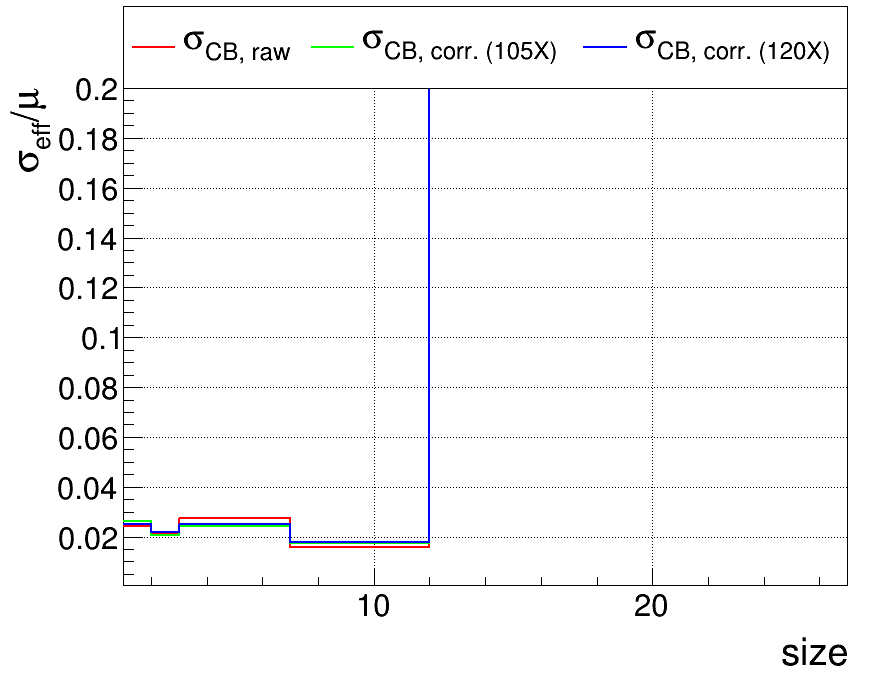
\includegraphics[width=0.495\textwidth]{EBFULL_CLUSSIZE_0005_0020_EffSigmaOverBins2.png}
\end{frame}

%%\begin{frame}[fragile]
\begin{verbatim}
EBFULL_CLUSSIZE_0005_0020_EffSigmaOverBins.png
\end{verbatim}
\includegraphics[width=0.495\textwidth]{plots_noPU/EBFULL_CLUSSIZE_0005_0020_EffSigmaOverBins.png}
\includegraphics[width=0.495\textwidth]{plots_noPU0.1/EBFULL_CLUSSIZE_0005_0020_EffSigmaOverBins.png}
\end{frame}
\begin{frame}[fragile]
\begin{verbatim}
EBFULL_CLUSSIZE_0005_0020_MuOverBins.png
\end{verbatim}
\includegraphics[width=0.495\textwidth]{plots_noPU/EBFULL_CLUSSIZE_0005_0020_MuOverBins.png}
\includegraphics[width=0.495\textwidth]{plots_noPU0.1/EBFULL_CLUSSIZE_0005_0020_MuOverBins.png}
\end{frame}
\begin{frame}[fragile]
\begin{verbatim}
EBFULL_CLUSSIZE_0005_0020_PerBinFitEcor74formula.png
\end{verbatim}
\includegraphics[width=0.495\textwidth]{plots_noPU/EBFULL_CLUSSIZE_0005_0020_PerBinFitEcor74formula.png}
\includegraphics[width=0.495\textwidth]{plots_noPU0.1/EBFULL_CLUSSIZE_0005_0020_PerBinFitEcor74formula.png}
\end{frame}
\begin{frame}[fragile]
\begin{verbatim}
EBFULL_CLUSSIZE_0005_0020_PerBinFitEcor91formula.png
\end{verbatim}
\includegraphics[width=0.495\textwidth]{plots_noPU/EBFULL_CLUSSIZE_0005_0020_PerBinFitEcor91formula.png}
\includegraphics[width=0.495\textwidth]{plots_noPU0.1/EBFULL_CLUSSIZE_0005_0020_PerBinFitEcor91formula.png}
\end{frame}
\begin{frame}[fragile]
\begin{verbatim}
EBFULL_CLUSSIZE_0005_0020_PerBinFitRawformula.png
\end{verbatim}
\includegraphics[width=0.495\textwidth]{plots_noPU/EBFULL_CLUSSIZE_0005_0020_PerBinFitRawformula.png}
\includegraphics[width=0.495\textwidth]{plots_noPU0.1/EBFULL_CLUSSIZE_0005_0020_PerBinFitRawformula.png}
\end{frame}
\begin{frame}[fragile]
\begin{verbatim}
EBFULL_CLUSSIZE_0020_0100_EffSigmaOverBins.png
\end{verbatim}
\includegraphics[width=0.495\textwidth]{plots_noPU/EBFULL_CLUSSIZE_0020_0100_EffSigmaOverBins.png}
\includegraphics[width=0.495\textwidth]{plots_noPU0.1/EBFULL_CLUSSIZE_0020_0100_EffSigmaOverBins.png}
\end{frame}
\begin{frame}[fragile]
\begin{verbatim}
EBFULL_CLUSSIZE_0020_0100_MuOverBins.png
\end{verbatim}
\includegraphics[width=0.495\textwidth]{plots_noPU/EBFULL_CLUSSIZE_0020_0100_MuOverBins.png}
\includegraphics[width=0.495\textwidth]{plots_noPU0.1/EBFULL_CLUSSIZE_0020_0100_MuOverBins.png}
\end{frame}
\begin{frame}[fragile]
\begin{verbatim}
EBFULL_CLUSSIZE_0020_0100_PerBinFitEcor74formula.png
\end{verbatim}
\includegraphics[width=0.495\textwidth]{plots_noPU/EBFULL_CLUSSIZE_0020_0100_PerBinFitEcor74formula.png}
\includegraphics[width=0.495\textwidth]{plots_noPU0.1/EBFULL_CLUSSIZE_0020_0100_PerBinFitEcor74formula.png}
\end{frame}
\begin{frame}[fragile]
\begin{verbatim}
EBFULL_CLUSSIZE_0020_0100_PerBinFitEcor91formula.png
\end{verbatim}
\includegraphics[width=0.495\textwidth]{plots_noPU/EBFULL_CLUSSIZE_0020_0100_PerBinFitEcor91formula.png}
\includegraphics[width=0.495\textwidth]{plots_noPU0.1/EBFULL_CLUSSIZE_0020_0100_PerBinFitEcor91formula.png}
\end{frame}
\begin{frame}[fragile]
\begin{verbatim}
EBFULL_CLUSSIZE_0020_0100_PerBinFitRawformula.png
\end{verbatim}
\includegraphics[width=0.495\textwidth]{plots_noPU/EBFULL_CLUSSIZE_0020_0100_PerBinFitRawformula.png}
\includegraphics[width=0.495\textwidth]{plots_noPU0.1/EBFULL_CLUSSIZE_0020_0100_PerBinFitRawformula.png}
\end{frame}
\begin{frame}[fragile]
\begin{verbatim}
EBFULL_CLUSSIZE_0100_0300_EffSigmaOverBins.png
\end{verbatim}
\includegraphics[width=0.495\textwidth]{plots_noPU/EBFULL_CLUSSIZE_0100_0300_EffSigmaOverBins.png}
\includegraphics[width=0.495\textwidth]{plots_noPU0.1/EBFULL_CLUSSIZE_0100_0300_EffSigmaOverBins.png}
\end{frame}
\begin{frame}[fragile]
\begin{verbatim}
EBFULL_CLUSSIZE_0100_0300_MuOverBins.png
\end{verbatim}
\includegraphics[width=0.495\textwidth]{plots_noPU/EBFULL_CLUSSIZE_0100_0300_MuOverBins.png}
\includegraphics[width=0.495\textwidth]{plots_noPU0.1/EBFULL_CLUSSIZE_0100_0300_MuOverBins.png}
\end{frame}
\begin{frame}[fragile]
\begin{verbatim}
EBFULL_CLUSSIZE_0100_0300_PerBinFitEcor74formula.png
\end{verbatim}
\includegraphics[width=0.495\textwidth]{plots_noPU/EBFULL_CLUSSIZE_0100_0300_PerBinFitEcor74formula.png}
\includegraphics[width=0.495\textwidth]{plots_noPU0.1/EBFULL_CLUSSIZE_0100_0300_PerBinFitEcor74formula.png}
\end{frame}
\begin{frame}[fragile]
\begin{verbatim}
EBFULL_CLUSSIZE_0100_0300_PerBinFitEcor91formula.png
\end{verbatim}
\includegraphics[width=0.495\textwidth]{plots_noPU/EBFULL_CLUSSIZE_0100_0300_PerBinFitEcor91formula.png}
\includegraphics[width=0.495\textwidth]{plots_noPU0.1/EBFULL_CLUSSIZE_0100_0300_PerBinFitEcor91formula.png}
\end{frame}
\begin{frame}[fragile]
\begin{verbatim}
EBFULL_CLUSSIZE_0100_0300_PerBinFitRawformula.png
\end{verbatim}
\includegraphics[width=0.495\textwidth]{plots_noPU/EBFULL_CLUSSIZE_0100_0300_PerBinFitRawformula.png}
\includegraphics[width=0.495\textwidth]{plots_noPU0.1/EBFULL_CLUSSIZE_0100_0300_PerBinFitRawformula.png}
\end{frame}
\begin{frame}[fragile]
\begin{verbatim}
EBFULL_GENETA_0005_0020_EffSigmaOverBins.png
\end{verbatim}
\includegraphics[width=0.495\textwidth]{plots_noPU/EBFULL_GENETA_0005_0020_EffSigmaOverBins.png}
\includegraphics[width=0.495\textwidth]{plots_noPU0.1/EBFULL_GENETA_0005_0020_EffSigmaOverBins.png}
\end{frame}
\begin{frame}[fragile]
\begin{verbatim}
EBFULL_GENETA_0005_0020_MuOverBins.png
\end{verbatim}
\includegraphics[width=0.495\textwidth]{plots_noPU/EBFULL_GENETA_0005_0020_MuOverBins.png}
\includegraphics[width=0.495\textwidth]{plots_noPU0.1/EBFULL_GENETA_0005_0020_MuOverBins.png}
\end{frame}
\begin{frame}[fragile]
\begin{verbatim}
EBFULL_GENETA_0005_0020_PerBinFitEcor74formula.png
\end{verbatim}
\includegraphics[width=0.495\textwidth]{plots_noPU/EBFULL_GENETA_0005_0020_PerBinFitEcor74formula.png}
\includegraphics[width=0.495\textwidth]{plots_noPU0.1/EBFULL_GENETA_0005_0020_PerBinFitEcor74formula.png}
\end{frame}
\begin{frame}[fragile]
\begin{verbatim}
EBFULL_GENETA_0005_0020_PerBinFitEcor91formula.png
\end{verbatim}
\includegraphics[width=0.495\textwidth]{plots_noPU/EBFULL_GENETA_0005_0020_PerBinFitEcor91formula.png}
\includegraphics[width=0.495\textwidth]{plots_noPU0.1/EBFULL_GENETA_0005_0020_PerBinFitEcor91formula.png}
\end{frame}
\begin{frame}[fragile]
\begin{verbatim}
EBFULL_GENETA_0005_0020_PerBinFitRawformula.png
\end{verbatim}
\includegraphics[width=0.495\textwidth]{plots_noPU/EBFULL_GENETA_0005_0020_PerBinFitRawformula.png}
\includegraphics[width=0.495\textwidth]{plots_noPU0.1/EBFULL_GENETA_0005_0020_PerBinFitRawformula.png}
\end{frame}
\begin{frame}[fragile]
\begin{verbatim}
EBFULL_GENETA_0020_0100_EffSigmaOverBins.png
\end{verbatim}
\includegraphics[width=0.495\textwidth]{plots_noPU/EBFULL_GENETA_0020_0100_EffSigmaOverBins.png}
\includegraphics[width=0.495\textwidth]{plots_noPU0.1/EBFULL_GENETA_0020_0100_EffSigmaOverBins.png}
\end{frame}
\begin{frame}[fragile]
\begin{verbatim}
EBFULL_GENETA_0020_0100_MuOverBins.png
\end{verbatim}
\includegraphics[width=0.495\textwidth]{plots_noPU/EBFULL_GENETA_0020_0100_MuOverBins.png}
\includegraphics[width=0.495\textwidth]{plots_noPU0.1/EBFULL_GENETA_0020_0100_MuOverBins.png}
\end{frame}
\begin{frame}[fragile]
\begin{verbatim}
EBFULL_GENETA_0020_0100_PerBinFitEcor74formula.png
\end{verbatim}
\includegraphics[width=0.495\textwidth]{plots_noPU/EBFULL_GENETA_0020_0100_PerBinFitEcor74formula.png}
\includegraphics[width=0.495\textwidth]{plots_noPU0.1/EBFULL_GENETA_0020_0100_PerBinFitEcor74formula.png}
\end{frame}
\begin{frame}[fragile]
\begin{verbatim}
EBFULL_GENETA_0020_0100_PerBinFitEcor91formula.png
\end{verbatim}
\includegraphics[width=0.495\textwidth]{plots_noPU/EBFULL_GENETA_0020_0100_PerBinFitEcor91formula.png}
\includegraphics[width=0.495\textwidth]{plots_noPU0.1/EBFULL_GENETA_0020_0100_PerBinFitEcor91formula.png}
\end{frame}
\begin{frame}[fragile]
\begin{verbatim}
EBFULL_GENETA_0020_0100_PerBinFitRawformula.png
\end{verbatim}
\includegraphics[width=0.495\textwidth]{plots_noPU/EBFULL_GENETA_0020_0100_PerBinFitRawformula.png}
\includegraphics[width=0.495\textwidth]{plots_noPU0.1/EBFULL_GENETA_0020_0100_PerBinFitRawformula.png}
\end{frame}
\begin{frame}[fragile]
\begin{verbatim}
EBFULL_GENETA_0100_0300_EffSigmaOverBins.png
\end{verbatim}
\includegraphics[width=0.495\textwidth]{plots_noPU/EBFULL_GENETA_0100_0300_EffSigmaOverBins.png}
\includegraphics[width=0.495\textwidth]{plots_noPU0.1/EBFULL_GENETA_0100_0300_EffSigmaOverBins.png}
\end{frame}
\begin{frame}[fragile]
\begin{verbatim}
EBFULL_GENETA_0100_0300_MuOverBins.png
\end{verbatim}
\includegraphics[width=0.495\textwidth]{plots_noPU/EBFULL_GENETA_0100_0300_MuOverBins.png}
\includegraphics[width=0.495\textwidth]{plots_noPU0.1/EBFULL_GENETA_0100_0300_MuOverBins.png}
\end{frame}
\begin{frame}[fragile]
\begin{verbatim}
EBFULL_GENETA_0100_0300_PerBinFitEcor74formula.png
\end{verbatim}
\includegraphics[width=0.495\textwidth]{plots_noPU/EBFULL_GENETA_0100_0300_PerBinFitEcor74formula.png}
\includegraphics[width=0.495\textwidth]{plots_noPU0.1/EBFULL_GENETA_0100_0300_PerBinFitEcor74formula.png}
\end{frame}
\begin{frame}[fragile]
\begin{verbatim}
EBFULL_GENETA_0100_0300_PerBinFitEcor91formula.png
\end{verbatim}
\includegraphics[width=0.495\textwidth]{plots_noPU/EBFULL_GENETA_0100_0300_PerBinFitEcor91formula.png}
\includegraphics[width=0.495\textwidth]{plots_noPU0.1/EBFULL_GENETA_0100_0300_PerBinFitEcor91formula.png}
\end{frame}
\begin{frame}[fragile]
\begin{verbatim}
EBFULL_GENETA_0100_0300_PerBinFitRawformula.png
\end{verbatim}
\includegraphics[width=0.495\textwidth]{plots_noPU/EBFULL_GENETA_0100_0300_PerBinFitRawformula.png}
\includegraphics[width=0.495\textwidth]{plots_noPU0.1/EBFULL_GENETA_0100_0300_PerBinFitRawformula.png}
\end{frame}
\begin{frame}[fragile]
\begin{verbatim}
EBFULL_GENPT_0005_0020_EffSigmaOverBins.png
\end{verbatim}
\includegraphics[width=0.495\textwidth]{plots_noPU/EBFULL_GENPT_0005_0020_EffSigmaOverBins.png}
\includegraphics[width=0.495\textwidth]{plots_noPU0.1/EBFULL_GENPT_0005_0020_EffSigmaOverBins.png}
\end{frame}
\begin{frame}[fragile]
\begin{verbatim}
EBFULL_GENPT_0005_0020_MuOverBins.png
\end{verbatim}
\includegraphics[width=0.495\textwidth]{plots_noPU/EBFULL_GENPT_0005_0020_MuOverBins.png}
\includegraphics[width=0.495\textwidth]{plots_noPU0.1/EBFULL_GENPT_0005_0020_MuOverBins.png}
\end{frame}
\begin{frame}[fragile]
\begin{verbatim}
EBFULL_GENPT_0005_0020_PerBinFitEcor74formula.png
\end{verbatim}
\includegraphics[width=0.495\textwidth]{plots_noPU/EBFULL_GENPT_0005_0020_PerBinFitEcor74formula.png}
\includegraphics[width=0.495\textwidth]{plots_noPU0.1/EBFULL_GENPT_0005_0020_PerBinFitEcor74formula.png}
\end{frame}
\begin{frame}[fragile]
\begin{verbatim}
EBFULL_GENPT_0005_0020_PerBinFitEcor91formula.png
\end{verbatim}
\includegraphics[width=0.495\textwidth]{plots_noPU/EBFULL_GENPT_0005_0020_PerBinFitEcor91formula.png}
\includegraphics[width=0.495\textwidth]{plots_noPU0.1/EBFULL_GENPT_0005_0020_PerBinFitEcor91formula.png}
\end{frame}
\begin{frame}[fragile]
\begin{verbatim}
EBFULL_GENPT_0005_0020_PerBinFitRawformula.png
\end{verbatim}
\includegraphics[width=0.495\textwidth]{plots_noPU/EBFULL_GENPT_0005_0020_PerBinFitRawformula.png}
\includegraphics[width=0.495\textwidth]{plots_noPU0.1/EBFULL_GENPT_0005_0020_PerBinFitRawformula.png}
\end{frame}
\begin{frame}[fragile]
\begin{verbatim}
EBFULL_GENPT_0020_0100_EffSigmaOverBins.png
\end{verbatim}
\includegraphics[width=0.495\textwidth]{plots_noPU/EBFULL_GENPT_0020_0100_EffSigmaOverBins.png}
\includegraphics[width=0.495\textwidth]{plots_noPU0.1/EBFULL_GENPT_0020_0100_EffSigmaOverBins.png}
\end{frame}
\begin{frame}[fragile]
\begin{verbatim}
EBFULL_GENPT_0020_0100_MuOverBins.png
\end{verbatim}
\includegraphics[width=0.495\textwidth]{plots_noPU/EBFULL_GENPT_0020_0100_MuOverBins.png}
\includegraphics[width=0.495\textwidth]{plots_noPU0.1/EBFULL_GENPT_0020_0100_MuOverBins.png}
\end{frame}
\begin{frame}[fragile]
\begin{verbatim}
EBFULL_GENPT_0020_0100_PerBinFitEcor74formula.png
\end{verbatim}
\includegraphics[width=0.495\textwidth]{plots_noPU/EBFULL_GENPT_0020_0100_PerBinFitEcor74formula.png}
\includegraphics[width=0.495\textwidth]{plots_noPU0.1/EBFULL_GENPT_0020_0100_PerBinFitEcor74formula.png}
\end{frame}
\begin{frame}[fragile]
\begin{verbatim}
EBFULL_GENPT_0020_0100_PerBinFitEcor91formula.png
\end{verbatim}
\includegraphics[width=0.495\textwidth]{plots_noPU/EBFULL_GENPT_0020_0100_PerBinFitEcor91formula.png}
\includegraphics[width=0.495\textwidth]{plots_noPU0.1/EBFULL_GENPT_0020_0100_PerBinFitEcor91formula.png}
\end{frame}
\begin{frame}[fragile]
\begin{verbatim}
EBFULL_GENPT_0020_0100_PerBinFitRawformula.png
\end{verbatim}
\includegraphics[width=0.495\textwidth]{plots_noPU/EBFULL_GENPT_0020_0100_PerBinFitRawformula.png}
\includegraphics[width=0.495\textwidth]{plots_noPU0.1/EBFULL_GENPT_0020_0100_PerBinFitRawformula.png}
\end{frame}
\begin{frame}[fragile]
\begin{verbatim}
EBFULL_GENPT_0100_0300_EffSigmaOverBins.png
\end{verbatim}
\includegraphics[width=0.495\textwidth]{plots_noPU/EBFULL_GENPT_0100_0300_EffSigmaOverBins.png}
\includegraphics[width=0.495\textwidth]{plots_noPU0.1/EBFULL_GENPT_0100_0300_EffSigmaOverBins.png}
\end{frame}
\begin{frame}[fragile]
\begin{verbatim}
EBFULL_GENPT_0100_0300_MuOverBins.png
\end{verbatim}
\includegraphics[width=0.495\textwidth]{plots_noPU/EBFULL_GENPT_0100_0300_MuOverBins.png}
\includegraphics[width=0.495\textwidth]{plots_noPU0.1/EBFULL_GENPT_0100_0300_MuOverBins.png}
\end{frame}
\begin{frame}[fragile]
\begin{verbatim}
EBFULL_GENPT_0100_0300_PerBinFitEcor74formula.png
\end{verbatim}
\includegraphics[width=0.495\textwidth]{plots_noPU/EBFULL_GENPT_0100_0300_PerBinFitEcor74formula.png}
\includegraphics[width=0.495\textwidth]{plots_noPU0.1/EBFULL_GENPT_0100_0300_PerBinFitEcor74formula.png}
\end{frame}
\begin{frame}[fragile]
\begin{verbatim}
EBFULL_GENPT_0100_0300_PerBinFitEcor91formula.png
\end{verbatim}
\includegraphics[width=0.495\textwidth]{plots_noPU/EBFULL_GENPT_0100_0300_PerBinFitEcor91formula.png}
\includegraphics[width=0.495\textwidth]{plots_noPU0.1/EBFULL_GENPT_0100_0300_PerBinFitEcor91formula.png}
\end{frame}
\begin{frame}[fragile]
\begin{verbatim}
EBFULL_GENPT_0100_0300_PerBinFitRawformula.png
\end{verbatim}
\includegraphics[width=0.495\textwidth]{plots_noPU/EBFULL_GENPT_0100_0300_PerBinFitRawformula.png}
\includegraphics[width=0.495\textwidth]{plots_noPU0.1/EBFULL_GENPT_0100_0300_PerBinFitRawformula.png}
\end{frame}
\begin{frame}[fragile]
\begin{verbatim}
EBFULL_NVTX_0005_0020_EffSigmaOverBins.png
\end{verbatim}
\includegraphics[width=0.495\textwidth]{plots_noPU/EBFULL_NVTX_0005_0020_EffSigmaOverBins.png}
\includegraphics[width=0.495\textwidth]{plots_noPU0.1/EBFULL_NVTX_0005_0020_EffSigmaOverBins.png}
\end{frame}
\begin{frame}[fragile]
\begin{verbatim}
EBFULL_NVTX_0005_0020_MuOverBins.png
\end{verbatim}
\includegraphics[width=0.495\textwidth]{plots_noPU/EBFULL_NVTX_0005_0020_MuOverBins.png}
\includegraphics[width=0.495\textwidth]{plots_noPU0.1/EBFULL_NVTX_0005_0020_MuOverBins.png}
\end{frame}
\begin{frame}[fragile]
\begin{verbatim}
EBFULL_NVTX_0005_0020_PerBinFitEcor74formula.png
\end{verbatim}
\includegraphics[width=0.495\textwidth]{plots_noPU/EBFULL_NVTX_0005_0020_PerBinFitEcor74formula.png}
\includegraphics[width=0.495\textwidth]{plots_noPU0.1/EBFULL_NVTX_0005_0020_PerBinFitEcor74formula.png}
\end{frame}
\begin{frame}[fragile]
\begin{verbatim}
EBFULL_NVTX_0005_0020_PerBinFitEcor91formula.png
\end{verbatim}
\includegraphics[width=0.495\textwidth]{plots_noPU/EBFULL_NVTX_0005_0020_PerBinFitEcor91formula.png}
\includegraphics[width=0.495\textwidth]{plots_noPU0.1/EBFULL_NVTX_0005_0020_PerBinFitEcor91formula.png}
\end{frame}
\begin{frame}[fragile]
\begin{verbatim}
EBFULL_NVTX_0005_0020_PerBinFitRawformula.png
\end{verbatim}
\includegraphics[width=0.495\textwidth]{plots_noPU/EBFULL_NVTX_0005_0020_PerBinFitRawformula.png}
\includegraphics[width=0.495\textwidth]{plots_noPU0.1/EBFULL_NVTX_0005_0020_PerBinFitRawformula.png}
\end{frame}
\begin{frame}[fragile]
\begin{verbatim}
EBFULL_NVTX_0020_0100_EffSigmaOverBins.png
\end{verbatim}
\includegraphics[width=0.495\textwidth]{plots_noPU/EBFULL_NVTX_0020_0100_EffSigmaOverBins.png}
\includegraphics[width=0.495\textwidth]{plots_noPU0.1/EBFULL_NVTX_0020_0100_EffSigmaOverBins.png}
\end{frame}
\begin{frame}[fragile]
\begin{verbatim}
EBFULL_NVTX_0020_0100_MuOverBins.png
\end{verbatim}
\includegraphics[width=0.495\textwidth]{plots_noPU/EBFULL_NVTX_0020_0100_MuOverBins.png}
\includegraphics[width=0.495\textwidth]{plots_noPU0.1/EBFULL_NVTX_0020_0100_MuOverBins.png}
\end{frame}
\begin{frame}[fragile]
\begin{verbatim}
EBFULL_NVTX_0020_0100_PerBinFitEcor74formula.png
\end{verbatim}
\includegraphics[width=0.495\textwidth]{plots_noPU/EBFULL_NVTX_0020_0100_PerBinFitEcor74formula.png}
\includegraphics[width=0.495\textwidth]{plots_noPU0.1/EBFULL_NVTX_0020_0100_PerBinFitEcor74formula.png}
\end{frame}
\begin{frame}[fragile]
\begin{verbatim}
EBFULL_NVTX_0020_0100_PerBinFitEcor91formula.png
\end{verbatim}
\includegraphics[width=0.495\textwidth]{plots_noPU/EBFULL_NVTX_0020_0100_PerBinFitEcor91formula.png}
\includegraphics[width=0.495\textwidth]{plots_noPU0.1/EBFULL_NVTX_0020_0100_PerBinFitEcor91formula.png}
\end{frame}
\begin{frame}[fragile]
\begin{verbatim}
EBFULL_NVTX_0020_0100_PerBinFitRawformula.png
\end{verbatim}
\includegraphics[width=0.495\textwidth]{plots_noPU/EBFULL_NVTX_0020_0100_PerBinFitRawformula.png}
\includegraphics[width=0.495\textwidth]{plots_noPU0.1/EBFULL_NVTX_0020_0100_PerBinFitRawformula.png}
\end{frame}
\begin{frame}[fragile]
\begin{verbatim}
EBFULL_NVTX_0100_0300_EffSigmaOverBins.png
\end{verbatim}
\includegraphics[width=0.495\textwidth]{plots_noPU/EBFULL_NVTX_0100_0300_EffSigmaOverBins.png}
\includegraphics[width=0.495\textwidth]{plots_noPU0.1/EBFULL_NVTX_0100_0300_EffSigmaOverBins.png}
\end{frame}
\begin{frame}[fragile]
\begin{verbatim}
EBFULL_NVTX_0100_0300_MuOverBins.png
\end{verbatim}
\includegraphics[width=0.495\textwidth]{plots_noPU/EBFULL_NVTX_0100_0300_MuOverBins.png}
\includegraphics[width=0.495\textwidth]{plots_noPU0.1/EBFULL_NVTX_0100_0300_MuOverBins.png}
\end{frame}
\begin{frame}[fragile]
\begin{verbatim}
EBFULL_NVTX_0100_0300_PerBinFitEcor74formula.png
\end{verbatim}
\includegraphics[width=0.495\textwidth]{plots_noPU/EBFULL_NVTX_0100_0300_PerBinFitEcor74formula.png}
\includegraphics[width=0.495\textwidth]{plots_noPU0.1/EBFULL_NVTX_0100_0300_PerBinFitEcor74formula.png}
\end{frame}
\begin{frame}[fragile]
\begin{verbatim}
EBFULL_NVTX_0100_0300_PerBinFitEcor91formula.png
\end{verbatim}
\includegraphics[width=0.495\textwidth]{plots_noPU/EBFULL_NVTX_0100_0300_PerBinFitEcor91formula.png}
\includegraphics[width=0.495\textwidth]{plots_noPU0.1/EBFULL_NVTX_0100_0300_PerBinFitEcor91formula.png}
\end{frame}
\begin{frame}[fragile]
\begin{verbatim}
EBFULL_NVTX_0100_0300_PerBinFitRawformula.png
\end{verbatim}
\includegraphics[width=0.495\textwidth]{plots_noPU/EBFULL_NVTX_0100_0300_PerBinFitRawformula.png}
\includegraphics[width=0.495\textwidth]{plots_noPU0.1/EBFULL_NVTX_0100_0300_PerBinFitRawformula.png}
\end{frame}
\begin{frame}[fragile]
\begin{verbatim}
EBFULL_iETA_0002_0005_EffSigmaOverBins.png
\end{verbatim}
\includegraphics[width=0.495\textwidth]{plots_noPU/EBFULL_iETA_0002_0005_EffSigmaOverBins.png}
\includegraphics[width=0.495\textwidth]{plots_noPU0.1/EBFULL_iETA_0002_0005_EffSigmaOverBins.png}
\end{frame}
\begin{frame}[fragile]
\begin{verbatim}
EBFULL_iETA_0002_0005_MuOverBins.png
\end{verbatim}
\includegraphics[width=0.495\textwidth]{plots_noPU/EBFULL_iETA_0002_0005_MuOverBins.png}
\includegraphics[width=0.495\textwidth]{plots_noPU0.1/EBFULL_iETA_0002_0005_MuOverBins.png}
\end{frame}
\begin{frame}[fragile]
\begin{verbatim}
EBFULL_iETA_0002_0005_PerBinFitEcor74formula.png
\end{verbatim}
\includegraphics[width=0.495\textwidth]{plots_noPU/EBFULL_iETA_0002_0005_PerBinFitEcor74formula.png}
\includegraphics[width=0.495\textwidth]{plots_noPU0.1/EBFULL_iETA_0002_0005_PerBinFitEcor74formula.png}
\end{frame}
\begin{frame}[fragile]
\begin{verbatim}
EBFULL_iETA_0002_0005_PerBinFitEcor91formula.png
\end{verbatim}
\includegraphics[width=0.495\textwidth]{plots_noPU/EBFULL_iETA_0002_0005_PerBinFitEcor91formula.png}
\includegraphics[width=0.495\textwidth]{plots_noPU0.1/EBFULL_iETA_0002_0005_PerBinFitEcor91formula.png}
\end{frame}
\begin{frame}[fragile]
\begin{verbatim}
EBFULL_iETA_0002_0005_PerBinFitRawformula.png
\end{verbatim}
\includegraphics[width=0.495\textwidth]{plots_noPU/EBFULL_iETA_0002_0005_PerBinFitRawformula.png}
\includegraphics[width=0.495\textwidth]{plots_noPU0.1/EBFULL_iETA_0002_0005_PerBinFitRawformula.png}
\end{frame}
\begin{frame}[fragile]
\begin{verbatim}
EBFULL_iETA_0005_0020_EffSigmaOverBins.png
\end{verbatim}
\includegraphics[width=0.495\textwidth]{plots_noPU/EBFULL_iETA_0005_0020_EffSigmaOverBins.png}
\includegraphics[width=0.495\textwidth]{plots_noPU0.1/EBFULL_iETA_0005_0020_EffSigmaOverBins.png}
\end{frame}
\begin{frame}[fragile]
\begin{verbatim}
EBFULL_iETA_0005_0020_MuOverBins.png
\end{verbatim}
\includegraphics[width=0.495\textwidth]{plots_noPU/EBFULL_iETA_0005_0020_MuOverBins.png}
\includegraphics[width=0.495\textwidth]{plots_noPU0.1/EBFULL_iETA_0005_0020_MuOverBins.png}
\end{frame}
\begin{frame}[fragile]
\begin{verbatim}
EBFULL_iETA_0005_0020_PerBinFitEcor74formula.png
\end{verbatim}
\includegraphics[width=0.495\textwidth]{plots_noPU/EBFULL_iETA_0005_0020_PerBinFitEcor74formula.png}
\includegraphics[width=0.495\textwidth]{plots_noPU0.1/EBFULL_iETA_0005_0020_PerBinFitEcor74formula.png}
\end{frame}
\begin{frame}[fragile]
\begin{verbatim}
EBFULL_iETA_0005_0020_PerBinFitEcor91formula.png
\end{verbatim}
\includegraphics[width=0.495\textwidth]{plots_noPU/EBFULL_iETA_0005_0020_PerBinFitEcor91formula.png}
\includegraphics[width=0.495\textwidth]{plots_noPU0.1/EBFULL_iETA_0005_0020_PerBinFitEcor91formula.png}
\end{frame}
\begin{frame}[fragile]
\begin{verbatim}
EBFULL_iETA_0005_0020_PerBinFitRawformula.png
\end{verbatim}
\includegraphics[width=0.495\textwidth]{plots_noPU/EBFULL_iETA_0005_0020_PerBinFitRawformula.png}
\includegraphics[width=0.495\textwidth]{plots_noPU0.1/EBFULL_iETA_0005_0020_PerBinFitRawformula.png}
\end{frame}
\begin{frame}[fragile]
\begin{verbatim}
EBFULL_iETA_0020_0100_EffSigmaOverBins.png
\end{verbatim}
\includegraphics[width=0.495\textwidth]{plots_noPU/EBFULL_iETA_0020_0100_EffSigmaOverBins.png}
\includegraphics[width=0.495\textwidth]{plots_noPU0.1/EBFULL_iETA_0020_0100_EffSigmaOverBins.png}
\end{frame}
\begin{frame}[fragile]
\begin{verbatim}
EBFULL_iETA_0020_0100_MuOverBins.png
\end{verbatim}
\includegraphics[width=0.495\textwidth]{plots_noPU/EBFULL_iETA_0020_0100_MuOverBins.png}
\includegraphics[width=0.495\textwidth]{plots_noPU0.1/EBFULL_iETA_0020_0100_MuOverBins.png}
\end{frame}
\begin{frame}[fragile]
\begin{verbatim}
EBFULL_iETA_0020_0100_PerBinFitEcor74formula.png
\end{verbatim}
\includegraphics[width=0.495\textwidth]{plots_noPU/EBFULL_iETA_0020_0100_PerBinFitEcor74formula.png}
\includegraphics[width=0.495\textwidth]{plots_noPU0.1/EBFULL_iETA_0020_0100_PerBinFitEcor74formula.png}
\end{frame}
\begin{frame}[fragile]
\begin{verbatim}
EBFULL_iETA_0020_0100_PerBinFitEcor91formula.png
\end{verbatim}
\includegraphics[width=0.495\textwidth]{plots_noPU/EBFULL_iETA_0020_0100_PerBinFitEcor91formula.png}
\includegraphics[width=0.495\textwidth]{plots_noPU0.1/EBFULL_iETA_0020_0100_PerBinFitEcor91formula.png}
\end{frame}
\begin{frame}[fragile]
\begin{verbatim}
EBFULL_iETA_0020_0100_PerBinFitRawformula.png
\end{verbatim}
\includegraphics[width=0.495\textwidth]{plots_noPU/EBFULL_iETA_0020_0100_PerBinFitRawformula.png}
\includegraphics[width=0.495\textwidth]{plots_noPU0.1/EBFULL_iETA_0020_0100_PerBinFitRawformula.png}
\end{frame}
\begin{frame}[fragile]
\begin{verbatim}
EBFULL_iETA_0100_0300_EffSigmaOverBins.png
\end{verbatim}
\includegraphics[width=0.495\textwidth]{plots_noPU/EBFULL_iETA_0100_0300_EffSigmaOverBins.png}
\includegraphics[width=0.495\textwidth]{plots_noPU0.1/EBFULL_iETA_0100_0300_EffSigmaOverBins.png}
\end{frame}
\begin{frame}[fragile]
\begin{verbatim}
EBFULL_iETA_0100_0300_MuOverBins.png
\end{verbatim}
\includegraphics[width=0.495\textwidth]{plots_noPU/EBFULL_iETA_0100_0300_MuOverBins.png}
\includegraphics[width=0.495\textwidth]{plots_noPU0.1/EBFULL_iETA_0100_0300_MuOverBins.png}
\end{frame}
\begin{frame}[fragile]
\begin{verbatim}
EBFULL_iETA_0100_0300_PerBinFitEcor74formula.png
\end{verbatim}
\includegraphics[width=0.495\textwidth]{plots_noPU/EBFULL_iETA_0100_0300_PerBinFitEcor74formula.png}
\includegraphics[width=0.495\textwidth]{plots_noPU0.1/EBFULL_iETA_0100_0300_PerBinFitEcor74formula.png}
\end{frame}
\begin{frame}[fragile]
\begin{verbatim}
EBFULL_iETA_0100_0300_PerBinFitEcor91formula.png
\end{verbatim}
\includegraphics[width=0.495\textwidth]{plots_noPU/EBFULL_iETA_0100_0300_PerBinFitEcor91formula.png}
\includegraphics[width=0.495\textwidth]{plots_noPU0.1/EBFULL_iETA_0100_0300_PerBinFitEcor91formula.png}
\end{frame}
\begin{frame}[fragile]
\begin{verbatim}
EBFULL_iETA_0100_0300_PerBinFitRawformula.png
\end{verbatim}
\includegraphics[width=0.495\textwidth]{plots_noPU/EBFULL_iETA_0100_0300_PerBinFitRawformula.png}
\includegraphics[width=0.495\textwidth]{plots_noPU0.1/EBFULL_iETA_0100_0300_PerBinFitRawformula.png}
\end{frame}
\begin{frame}[fragile]
\begin{verbatim}
EBFULL_iPHI_0002_0005_EffSigmaOverBins.png
\end{verbatim}
\includegraphics[width=0.495\textwidth]{plots_noPU/EBFULL_iPHI_0002_0005_EffSigmaOverBins.png}
\includegraphics[width=0.495\textwidth]{plots_noPU0.1/EBFULL_iPHI_0002_0005_EffSigmaOverBins.png}
\end{frame}
\begin{frame}[fragile]
\begin{verbatim}
EBFULL_iPHI_0002_0005_MuOverBins.png
\end{verbatim}
\includegraphics[width=0.495\textwidth]{plots_noPU/EBFULL_iPHI_0002_0005_MuOverBins.png}
\includegraphics[width=0.495\textwidth]{plots_noPU0.1/EBFULL_iPHI_0002_0005_MuOverBins.png}
\end{frame}
\begin{frame}[fragile]
\begin{verbatim}
EBFULL_iPHI_0002_0005_PerBinFitEcor74formula.png
\end{verbatim}
\includegraphics[width=0.495\textwidth]{plots_noPU/EBFULL_iPHI_0002_0005_PerBinFitEcor74formula.png}
\includegraphics[width=0.495\textwidth]{plots_noPU0.1/EBFULL_iPHI_0002_0005_PerBinFitEcor74formula.png}
\end{frame}
\begin{frame}[fragile]
\begin{verbatim}
EBFULL_iPHI_0002_0005_PerBinFitEcor91formula.png
\end{verbatim}
\includegraphics[width=0.495\textwidth]{plots_noPU/EBFULL_iPHI_0002_0005_PerBinFitEcor91formula.png}
\includegraphics[width=0.495\textwidth]{plots_noPU0.1/EBFULL_iPHI_0002_0005_PerBinFitEcor91formula.png}
\end{frame}
\begin{frame}[fragile]
\begin{verbatim}
EBFULL_iPHI_0002_0005_PerBinFitRawformula.png
\end{verbatim}
\includegraphics[width=0.495\textwidth]{plots_noPU/EBFULL_iPHI_0002_0005_PerBinFitRawformula.png}
\includegraphics[width=0.495\textwidth]{plots_noPU0.1/EBFULL_iPHI_0002_0005_PerBinFitRawformula.png}
\end{frame}
\begin{frame}[fragile]
\begin{verbatim}
EBFULL_iPHI_0005_0020_EffSigmaOverBins.png
\end{verbatim}
\includegraphics[width=0.495\textwidth]{plots_noPU/EBFULL_iPHI_0005_0020_EffSigmaOverBins.png}
\includegraphics[width=0.495\textwidth]{plots_noPU0.1/EBFULL_iPHI_0005_0020_EffSigmaOverBins.png}
\end{frame}
\begin{frame}[fragile]
\begin{verbatim}
EBFULL_iPHI_0005_0020_MuOverBins.png
\end{verbatim}
\includegraphics[width=0.495\textwidth]{plots_noPU/EBFULL_iPHI_0005_0020_MuOverBins.png}
\includegraphics[width=0.495\textwidth]{plots_noPU0.1/EBFULL_iPHI_0005_0020_MuOverBins.png}
\end{frame}
\begin{frame}[fragile]
\begin{verbatim}
EBFULL_iPHI_0005_0020_PerBinFitEcor74formula.png
\end{verbatim}
\includegraphics[width=0.495\textwidth]{plots_noPU/EBFULL_iPHI_0005_0020_PerBinFitEcor74formula.png}
\includegraphics[width=0.495\textwidth]{plots_noPU0.1/EBFULL_iPHI_0005_0020_PerBinFitEcor74formula.png}
\end{frame}
\begin{frame}[fragile]
\begin{verbatim}
EBFULL_iPHI_0005_0020_PerBinFitEcor91formula.png
\end{verbatim}
\includegraphics[width=0.495\textwidth]{plots_noPU/EBFULL_iPHI_0005_0020_PerBinFitEcor91formula.png}
\includegraphics[width=0.495\textwidth]{plots_noPU0.1/EBFULL_iPHI_0005_0020_PerBinFitEcor91formula.png}
\end{frame}
\begin{frame}[fragile]
\begin{verbatim}
EBFULL_iPHI_0005_0020_PerBinFitRawformula.png
\end{verbatim}
\includegraphics[width=0.495\textwidth]{plots_noPU/EBFULL_iPHI_0005_0020_PerBinFitRawformula.png}
\includegraphics[width=0.495\textwidth]{plots_noPU0.1/EBFULL_iPHI_0005_0020_PerBinFitRawformula.png}
\end{frame}
\begin{frame}[fragile]
\begin{verbatim}
EBFULL_iPHI_0020_0100_EffSigmaOverBins.png
\end{verbatim}
\includegraphics[width=0.495\textwidth]{plots_noPU/EBFULL_iPHI_0020_0100_EffSigmaOverBins.png}
\includegraphics[width=0.495\textwidth]{plots_noPU0.1/EBFULL_iPHI_0020_0100_EffSigmaOverBins.png}
\end{frame}
\begin{frame}[fragile]
\begin{verbatim}
EBFULL_iPHI_0020_0100_MuOverBins.png
\end{verbatim}
\includegraphics[width=0.495\textwidth]{plots_noPU/EBFULL_iPHI_0020_0100_MuOverBins.png}
\includegraphics[width=0.495\textwidth]{plots_noPU0.1/EBFULL_iPHI_0020_0100_MuOverBins.png}
\end{frame}
\begin{frame}[fragile]
\begin{verbatim}
EBFULL_iPHI_0020_0100_PerBinFitEcor74formula.png
\end{verbatim}
\includegraphics[width=0.495\textwidth]{plots_noPU/EBFULL_iPHI_0020_0100_PerBinFitEcor74formula.png}
\includegraphics[width=0.495\textwidth]{plots_noPU0.1/EBFULL_iPHI_0020_0100_PerBinFitEcor74formula.png}
\end{frame}
\begin{frame}[fragile]
\begin{verbatim}
EBFULL_iPHI_0020_0100_PerBinFitEcor91formula.png
\end{verbatim}
\includegraphics[width=0.495\textwidth]{plots_noPU/EBFULL_iPHI_0020_0100_PerBinFitEcor91formula.png}
\includegraphics[width=0.495\textwidth]{plots_noPU0.1/EBFULL_iPHI_0020_0100_PerBinFitEcor91formula.png}
\end{frame}
\begin{frame}[fragile]
\begin{verbatim}
EBFULL_iPHI_0020_0100_PerBinFitRawformula.png
\end{verbatim}
\includegraphics[width=0.495\textwidth]{plots_noPU/EBFULL_iPHI_0020_0100_PerBinFitRawformula.png}
\includegraphics[width=0.495\textwidth]{plots_noPU0.1/EBFULL_iPHI_0020_0100_PerBinFitRawformula.png}
\end{frame}
\begin{frame}[fragile]
\begin{verbatim}
EBFULL_iPHI_0100_0300_EffSigmaOverBins.png
\end{verbatim}
\includegraphics[width=0.495\textwidth]{plots_noPU/EBFULL_iPHI_0100_0300_EffSigmaOverBins.png}
\includegraphics[width=0.495\textwidth]{plots_noPU0.1/EBFULL_iPHI_0100_0300_EffSigmaOverBins.png}
\end{frame}
\begin{frame}[fragile]
\begin{verbatim}
EBFULL_iPHI_0100_0300_MuOverBins.png
\end{verbatim}
\includegraphics[width=0.495\textwidth]{plots_noPU/EBFULL_iPHI_0100_0300_MuOverBins.png}
\includegraphics[width=0.495\textwidth]{plots_noPU0.1/EBFULL_iPHI_0100_0300_MuOverBins.png}
\end{frame}
\begin{frame}[fragile]
\begin{verbatim}
EBFULL_iPHI_0100_0300_PerBinFitEcor74formula.png
\end{verbatim}
\includegraphics[width=0.495\textwidth]{plots_noPU/EBFULL_iPHI_0100_0300_PerBinFitEcor74formula.png}
\includegraphics[width=0.495\textwidth]{plots_noPU0.1/EBFULL_iPHI_0100_0300_PerBinFitEcor74formula.png}
\end{frame}
\begin{frame}[fragile]
\begin{verbatim}
EBFULL_iPHI_0100_0300_PerBinFitEcor91formula.png
\end{verbatim}
\includegraphics[width=0.495\textwidth]{plots_noPU/EBFULL_iPHI_0100_0300_PerBinFitEcor91formula.png}
\includegraphics[width=0.495\textwidth]{plots_noPU0.1/EBFULL_iPHI_0100_0300_PerBinFitEcor91formula.png}
\end{frame}
\begin{frame}[fragile]
\begin{verbatim}
EBFULL_iPHI_0100_0300_PerBinFitRawformula.png
\end{verbatim}
\includegraphics[width=0.495\textwidth]{plots_noPU/EBFULL_iPHI_0100_0300_PerBinFitRawformula.png}
\includegraphics[width=0.495\textwidth]{plots_noPU0.1/EBFULL_iPHI_0100_0300_PerBinFitRawformula.png}
\end{frame}
\begin{frame}[fragile]
\begin{verbatim}
EBZS_CLUSSIZE_0000_0006_EffSigmaOverBins.png
\end{verbatim}
\includegraphics[width=0.495\textwidth]{plots_noPU/EBZS_CLUSSIZE_0000_0006_EffSigmaOverBins.png}
\includegraphics[width=0.495\textwidth]{plots_noPU0.1/EBZS_CLUSSIZE_0000_0006_EffSigmaOverBins.png}
\end{frame}
\begin{frame}[fragile]
\begin{verbatim}
EBZS_CLUSSIZE_0000_0006_MuOverBins.png
\end{verbatim}
\includegraphics[width=0.495\textwidth]{plots_noPU/EBZS_CLUSSIZE_0000_0006_MuOverBins.png}
\includegraphics[width=0.495\textwidth]{plots_noPU0.1/EBZS_CLUSSIZE_0000_0006_MuOverBins.png}
\end{frame}
\begin{frame}[fragile]
\begin{verbatim}
EBZS_CLUSSIZE_0000_0006_PerBinFitEcor74formula.png
\end{verbatim}
\includegraphics[width=0.495\textwidth]{plots_noPU/EBZS_CLUSSIZE_0000_0006_PerBinFitEcor74formula.png}
\includegraphics[width=0.495\textwidth]{plots_noPU0.1/EBZS_CLUSSIZE_0000_0006_PerBinFitEcor74formula.png}
\end{frame}
\begin{frame}[fragile]
\begin{verbatim}
EBZS_CLUSSIZE_0000_0006_PerBinFitEcor91formula.png
\end{verbatim}
\includegraphics[width=0.495\textwidth]{plots_noPU/EBZS_CLUSSIZE_0000_0006_PerBinFitEcor91formula.png}
\includegraphics[width=0.495\textwidth]{plots_noPU0.1/EBZS_CLUSSIZE_0000_0006_PerBinFitEcor91formula.png}
\end{frame}
\begin{frame}[fragile]
\begin{verbatim}
EBZS_CLUSSIZE_0000_0006_PerBinFitRawformula.png
\end{verbatim}
\includegraphics[width=0.495\textwidth]{plots_noPU/EBZS_CLUSSIZE_0000_0006_PerBinFitRawformula.png}
\includegraphics[width=0.495\textwidth]{plots_noPU0.1/EBZS_CLUSSIZE_0000_0006_PerBinFitRawformula.png}
\end{frame}
\begin{frame}[fragile]
\begin{verbatim}
EBZS_CLUSSIZE_0006_0025_MuOverBins.png
\end{verbatim}
\includegraphics[width=0.495\textwidth]{plots_noPU/EBZS_CLUSSIZE_0006_0025_MuOverBins.png}
\includegraphics[width=0.495\textwidth]{plots_noPU0.1/EBZS_CLUSSIZE_0006_0025_MuOverBins.png}
\end{frame}
\begin{frame}[fragile]
\begin{verbatim}
EBZS_CLUSSIZE_0006_0025_PerBinFitEcor74formula.png
\end{verbatim}
\includegraphics[width=0.495\textwidth]{plots_noPU/EBZS_CLUSSIZE_0006_0025_PerBinFitEcor74formula.png}
\includegraphics[width=0.495\textwidth]{plots_noPU0.1/EBZS_CLUSSIZE_0006_0025_PerBinFitEcor74formula.png}
\end{frame}
\begin{frame}[fragile]
\begin{verbatim}
EBZS_CLUSSIZE_0006_0025_PerBinFitEcor91formula.png
\end{verbatim}
\includegraphics[width=0.495\textwidth]{plots_noPU/EBZS_CLUSSIZE_0006_0025_PerBinFitEcor91formula.png}
\includegraphics[width=0.495\textwidth]{plots_noPU0.1/EBZS_CLUSSIZE_0006_0025_PerBinFitEcor91formula.png}
\end{frame}
\begin{frame}[fragile]
\begin{verbatim}
EBZS_CLUSSIZE_0006_0025_PerBinFitRawformula.png
\end{verbatim}
\includegraphics[width=0.495\textwidth]{plots_noPU/EBZS_CLUSSIZE_0006_0025_PerBinFitRawformula.png}
\includegraphics[width=0.495\textwidth]{plots_noPU0.1/EBZS_CLUSSIZE_0006_0025_PerBinFitRawformula.png}
\end{frame}
\begin{frame}[fragile]
\begin{verbatim}
EBZS_GENETA_0000_0006_EffSigmaOverBins.png
\end{verbatim}
\includegraphics[width=0.495\textwidth]{plots_noPU/EBZS_GENETA_0000_0006_EffSigmaOverBins.png}
\includegraphics[width=0.495\textwidth]{plots_noPU0.1/EBZS_GENETA_0000_0006_EffSigmaOverBins.png}
\end{frame}
\begin{frame}[fragile]
\begin{verbatim}
EBZS_GENETA_0000_0006_MuOverBins.png
\end{verbatim}
\includegraphics[width=0.495\textwidth]{plots_noPU/EBZS_GENETA_0000_0006_MuOverBins.png}
\includegraphics[width=0.495\textwidth]{plots_noPU0.1/EBZS_GENETA_0000_0006_MuOverBins.png}
\end{frame}
\begin{frame}[fragile]
\begin{verbatim}
EBZS_GENETA_0000_0006_PerBinFitEcor74formula.png
\end{verbatim}
\includegraphics[width=0.495\textwidth]{plots_noPU/EBZS_GENETA_0000_0006_PerBinFitEcor74formula.png}
\includegraphics[width=0.495\textwidth]{plots_noPU0.1/EBZS_GENETA_0000_0006_PerBinFitEcor74formula.png}
\end{frame}
\begin{frame}[fragile]
\begin{verbatim}
EBZS_GENETA_0000_0006_PerBinFitEcor91formula.png
\end{verbatim}
\includegraphics[width=0.495\textwidth]{plots_noPU/EBZS_GENETA_0000_0006_PerBinFitEcor91formula.png}
\includegraphics[width=0.495\textwidth]{plots_noPU0.1/EBZS_GENETA_0000_0006_PerBinFitEcor91formula.png}
\end{frame}
\begin{frame}[fragile]
\begin{verbatim}
EBZS_GENETA_0000_0006_PerBinFitRawformula.png
\end{verbatim}
\includegraphics[width=0.495\textwidth]{plots_noPU/EBZS_GENETA_0000_0006_PerBinFitRawformula.png}
\includegraphics[width=0.495\textwidth]{plots_noPU0.1/EBZS_GENETA_0000_0006_PerBinFitRawformula.png}
\end{frame}
\begin{frame}[fragile]
\begin{verbatim}
EBZS_GENETA_0006_0025_EffSigmaOverBins.png
\end{verbatim}
\includegraphics[width=0.495\textwidth]{plots_noPU/EBZS_GENETA_0006_0025_EffSigmaOverBins.png}
\includegraphics[width=0.495\textwidth]{plots_noPU0.1/EBZS_GENETA_0006_0025_EffSigmaOverBins.png}
\end{frame}
\begin{frame}[fragile]
\begin{verbatim}
EBZS_GENETA_0006_0025_MuOverBins.png
\end{verbatim}
\includegraphics[width=0.495\textwidth]{plots_noPU/EBZS_GENETA_0006_0025_MuOverBins.png}
\includegraphics[width=0.495\textwidth]{plots_noPU0.1/EBZS_GENETA_0006_0025_MuOverBins.png}
\end{frame}
\begin{frame}[fragile]
\begin{verbatim}
EBZS_GENETA_0006_0025_PerBinFitEcor74formula.png
\end{verbatim}
\includegraphics[width=0.495\textwidth]{plots_noPU/EBZS_GENETA_0006_0025_PerBinFitEcor74formula.png}
\includegraphics[width=0.495\textwidth]{plots_noPU0.1/EBZS_GENETA_0006_0025_PerBinFitEcor74formula.png}
\end{frame}
\begin{frame}[fragile]
\begin{verbatim}
EBZS_GENETA_0006_0025_PerBinFitEcor91formula.png
\end{verbatim}
\includegraphics[width=0.495\textwidth]{plots_noPU/EBZS_GENETA_0006_0025_PerBinFitEcor91formula.png}
\includegraphics[width=0.495\textwidth]{plots_noPU0.1/EBZS_GENETA_0006_0025_PerBinFitEcor91formula.png}
\end{frame}
\begin{frame}[fragile]
\begin{verbatim}
EBZS_GENETA_0006_0025_PerBinFitRawformula.png
\end{verbatim}
\includegraphics[width=0.495\textwidth]{plots_noPU/EBZS_GENETA_0006_0025_PerBinFitRawformula.png}
\includegraphics[width=0.495\textwidth]{plots_noPU0.1/EBZS_GENETA_0006_0025_PerBinFitRawformula.png}
\end{frame}
\begin{frame}[fragile]
\begin{verbatim}
EBZS_GENPT_0000_0006_EffSigmaOverBins.png
\end{verbatim}
\includegraphics[width=0.495\textwidth]{plots_noPU/EBZS_GENPT_0000_0006_EffSigmaOverBins.png}
\includegraphics[width=0.495\textwidth]{plots_noPU0.1/EBZS_GENPT_0000_0006_EffSigmaOverBins.png}
\end{frame}
\begin{frame}[fragile]
\begin{verbatim}
EBZS_GENPT_0000_0006_MuOverBins.png
\end{verbatim}
\includegraphics[width=0.495\textwidth]{plots_noPU/EBZS_GENPT_0000_0006_MuOverBins.png}
\includegraphics[width=0.495\textwidth]{plots_noPU0.1/EBZS_GENPT_0000_0006_MuOverBins.png}
\end{frame}
\begin{frame}[fragile]
\begin{verbatim}
EBZS_GENPT_0000_0006_PerBinFitEcor74formula.png
\end{verbatim}
\includegraphics[width=0.495\textwidth]{plots_noPU/EBZS_GENPT_0000_0006_PerBinFitEcor74formula.png}
\includegraphics[width=0.495\textwidth]{plots_noPU0.1/EBZS_GENPT_0000_0006_PerBinFitEcor74formula.png}
\end{frame}
\begin{frame}[fragile]
\begin{verbatim}
EBZS_GENPT_0000_0006_PerBinFitEcor91formula.png
\end{verbatim}
\includegraphics[width=0.495\textwidth]{plots_noPU/EBZS_GENPT_0000_0006_PerBinFitEcor91formula.png}
\includegraphics[width=0.495\textwidth]{plots_noPU0.1/EBZS_GENPT_0000_0006_PerBinFitEcor91formula.png}
\end{frame}
\begin{frame}[fragile]
\begin{verbatim}
EBZS_GENPT_0000_0006_PerBinFitRawformula.png
\end{verbatim}
\includegraphics[width=0.495\textwidth]{plots_noPU/EBZS_GENPT_0000_0006_PerBinFitRawformula.png}
\includegraphics[width=0.495\textwidth]{plots_noPU0.1/EBZS_GENPT_0000_0006_PerBinFitRawformula.png}
\end{frame}
\begin{frame}[fragile]
\begin{verbatim}
EBZS_GENPT_0006_0025_EffSigmaOverBins.png
\end{verbatim}
\includegraphics[width=0.495\textwidth]{plots_noPU/EBZS_GENPT_0006_0025_EffSigmaOverBins.png}
\includegraphics[width=0.495\textwidth]{plots_noPU0.1/EBZS_GENPT_0006_0025_EffSigmaOverBins.png}
\end{frame}
\begin{frame}[fragile]
\begin{verbatim}
EBZS_GENPT_0006_0025_MuOverBins.png
\end{verbatim}
\includegraphics[width=0.495\textwidth]{plots_noPU/EBZS_GENPT_0006_0025_MuOverBins.png}
\includegraphics[width=0.495\textwidth]{plots_noPU0.1/EBZS_GENPT_0006_0025_MuOverBins.png}
\end{frame}
\begin{frame}[fragile]
\begin{verbatim}
EBZS_GENPT_0006_0025_PerBinFitEcor74formula.png
\end{verbatim}
\includegraphics[width=0.495\textwidth]{plots_noPU/EBZS_GENPT_0006_0025_PerBinFitEcor74formula.png}
\includegraphics[width=0.495\textwidth]{plots_noPU0.1/EBZS_GENPT_0006_0025_PerBinFitEcor74formula.png}
\end{frame}
\begin{frame}[fragile]
\begin{verbatim}
EBZS_GENPT_0006_0025_PerBinFitEcor91formula.png
\end{verbatim}
\includegraphics[width=0.495\textwidth]{plots_noPU/EBZS_GENPT_0006_0025_PerBinFitEcor91formula.png}
\includegraphics[width=0.495\textwidth]{plots_noPU0.1/EBZS_GENPT_0006_0025_PerBinFitEcor91formula.png}
\end{frame}
\begin{frame}[fragile]
\begin{verbatim}
EBZS_GENPT_0006_0025_PerBinFitRawformula.png
\end{verbatim}
\includegraphics[width=0.495\textwidth]{plots_noPU/EBZS_GENPT_0006_0025_PerBinFitRawformula.png}
\includegraphics[width=0.495\textwidth]{plots_noPU0.1/EBZS_GENPT_0006_0025_PerBinFitRawformula.png}
\end{frame}
\begin{frame}[fragile]
\begin{verbatim}
EBZS_NVTX_0000_0006_EffSigmaOverBins.png
\end{verbatim}
\includegraphics[width=0.495\textwidth]{plots_noPU/EBZS_NVTX_0000_0006_EffSigmaOverBins.png}
\includegraphics[width=0.495\textwidth]{plots_noPU0.1/EBZS_NVTX_0000_0006_EffSigmaOverBins.png}
\end{frame}
\begin{frame}[fragile]
\begin{verbatim}
EBZS_NVTX_0000_0006_MuOverBins.png
\end{verbatim}
\includegraphics[width=0.495\textwidth]{plots_noPU/EBZS_NVTX_0000_0006_MuOverBins.png}
\includegraphics[width=0.495\textwidth]{plots_noPU0.1/EBZS_NVTX_0000_0006_MuOverBins.png}
\end{frame}
\begin{frame}[fragile]
\begin{verbatim}
EBZS_NVTX_0000_0006_PerBinFitEcor74formula.png
\end{verbatim}
\includegraphics[width=0.495\textwidth]{plots_noPU/EBZS_NVTX_0000_0006_PerBinFitEcor74formula.png}
\includegraphics[width=0.495\textwidth]{plots_noPU0.1/EBZS_NVTX_0000_0006_PerBinFitEcor74formula.png}
\end{frame}
\begin{frame}[fragile]
\begin{verbatim}
EBZS_NVTX_0000_0006_PerBinFitEcor91formula.png
\end{verbatim}
\includegraphics[width=0.495\textwidth]{plots_noPU/EBZS_NVTX_0000_0006_PerBinFitEcor91formula.png}
\includegraphics[width=0.495\textwidth]{plots_noPU0.1/EBZS_NVTX_0000_0006_PerBinFitEcor91formula.png}
\end{frame}
\begin{frame}[fragile]
\begin{verbatim}
EBZS_NVTX_0000_0006_PerBinFitRawformula.png
\end{verbatim}
\includegraphics[width=0.495\textwidth]{plots_noPU/EBZS_NVTX_0000_0006_PerBinFitRawformula.png}
\includegraphics[width=0.495\textwidth]{plots_noPU0.1/EBZS_NVTX_0000_0006_PerBinFitRawformula.png}
\end{frame}
\begin{frame}[fragile]
\begin{verbatim}
EBZS_NVTX_0006_0025_EffSigmaOverBins.png
\end{verbatim}
\includegraphics[width=0.495\textwidth]{plots_noPU/EBZS_NVTX_0006_0025_EffSigmaOverBins.png}
\includegraphics[width=0.495\textwidth]{plots_noPU0.1/EBZS_NVTX_0006_0025_EffSigmaOverBins.png}
\end{frame}
\begin{frame}[fragile]
\begin{verbatim}
EBZS_NVTX_0006_0025_MuOverBins.png
\end{verbatim}
\includegraphics[width=0.495\textwidth]{plots_noPU/EBZS_NVTX_0006_0025_MuOverBins.png}
\includegraphics[width=0.495\textwidth]{plots_noPU0.1/EBZS_NVTX_0006_0025_MuOverBins.png}
\end{frame}
\begin{frame}[fragile]
\begin{verbatim}
EBZS_NVTX_0006_0025_PerBinFitEcor74formula.png
\end{verbatim}
\includegraphics[width=0.495\textwidth]{plots_noPU/EBZS_NVTX_0006_0025_PerBinFitEcor74formula.png}
\includegraphics[width=0.495\textwidth]{plots_noPU0.1/EBZS_NVTX_0006_0025_PerBinFitEcor74formula.png}
\end{frame}
\begin{frame}[fragile]
\begin{verbatim}
EBZS_NVTX_0006_0025_PerBinFitEcor91formula.png
\end{verbatim}
\includegraphics[width=0.495\textwidth]{plots_noPU/EBZS_NVTX_0006_0025_PerBinFitEcor91formula.png}
\includegraphics[width=0.495\textwidth]{plots_noPU0.1/EBZS_NVTX_0006_0025_PerBinFitEcor91formula.png}
\end{frame}
\begin{frame}[fragile]
\begin{verbatim}
EBZS_NVTX_0006_0025_PerBinFitRawformula.png
\end{verbatim}
\includegraphics[width=0.495\textwidth]{plots_noPU/EBZS_NVTX_0006_0025_PerBinFitRawformula.png}
\includegraphics[width=0.495\textwidth]{plots_noPU0.1/EBZS_NVTX_0006_0025_PerBinFitRawformula.png}
\end{frame}
\begin{frame}[fragile]
\begin{verbatim}
EEFULL_CLUSSIZE_0005_0020_EffSigmaOverBins.png
\end{verbatim}
\includegraphics[width=0.495\textwidth]{plots_noPU/EEFULL_CLUSSIZE_0005_0020_EffSigmaOverBins.png}
\includegraphics[width=0.495\textwidth]{plots_noPU0.1/EEFULL_CLUSSIZE_0005_0020_EffSigmaOverBins.png}
\end{frame}
\begin{frame}[fragile]
\begin{verbatim}
EEFULL_CLUSSIZE_0005_0020_MuOverBins.png
\end{verbatim}
\includegraphics[width=0.495\textwidth]{plots_noPU/EEFULL_CLUSSIZE_0005_0020_MuOverBins.png}
\includegraphics[width=0.495\textwidth]{plots_noPU0.1/EEFULL_CLUSSIZE_0005_0020_MuOverBins.png}
\end{frame}
\begin{frame}[fragile]
\begin{verbatim}
EEFULL_CLUSSIZE_0005_0020_PerBinFitEcor74formula.png
\end{verbatim}
\includegraphics[width=0.495\textwidth]{plots_noPU/EEFULL_CLUSSIZE_0005_0020_PerBinFitEcor74formula.png}
\includegraphics[width=0.495\textwidth]{plots_noPU0.1/EEFULL_CLUSSIZE_0005_0020_PerBinFitEcor74formula.png}
\end{frame}
\begin{frame}[fragile]
\begin{verbatim}
EEFULL_CLUSSIZE_0005_0020_PerBinFitEcor91formula.png
\end{verbatim}
\includegraphics[width=0.495\textwidth]{plots_noPU/EEFULL_CLUSSIZE_0005_0020_PerBinFitEcor91formula.png}
\includegraphics[width=0.495\textwidth]{plots_noPU0.1/EEFULL_CLUSSIZE_0005_0020_PerBinFitEcor91formula.png}
\end{frame}
\begin{frame}[fragile]
\begin{verbatim}
EEFULL_CLUSSIZE_0005_0020_PerBinFitRawformula.png
\end{verbatim}
\includegraphics[width=0.495\textwidth]{plots_noPU/EEFULL_CLUSSIZE_0005_0020_PerBinFitRawformula.png}
\includegraphics[width=0.495\textwidth]{plots_noPU0.1/EEFULL_CLUSSIZE_0005_0020_PerBinFitRawformula.png}
\end{frame}
\begin{frame}[fragile]
\begin{verbatim}
EEFULL_CLUSSIZE_0020_0100_EffSigmaOverBins.png
\end{verbatim}
\includegraphics[width=0.495\textwidth]{plots_noPU/EEFULL_CLUSSIZE_0020_0100_EffSigmaOverBins.png}
\includegraphics[width=0.495\textwidth]{plots_noPU0.1/EEFULL_CLUSSIZE_0020_0100_EffSigmaOverBins.png}
\end{frame}
\begin{frame}[fragile]
\begin{verbatim}
EEFULL_CLUSSIZE_0020_0100_MuOverBins.png
\end{verbatim}
\includegraphics[width=0.495\textwidth]{plots_noPU/EEFULL_CLUSSIZE_0020_0100_MuOverBins.png}
\includegraphics[width=0.495\textwidth]{plots_noPU0.1/EEFULL_CLUSSIZE_0020_0100_MuOverBins.png}
\end{frame}
\begin{frame}[fragile]
\begin{verbatim}
EEFULL_CLUSSIZE_0020_0100_PerBinFitEcor74formula.png
\end{verbatim}
\includegraphics[width=0.495\textwidth]{plots_noPU/EEFULL_CLUSSIZE_0020_0100_PerBinFitEcor74formula.png}
\includegraphics[width=0.495\textwidth]{plots_noPU0.1/EEFULL_CLUSSIZE_0020_0100_PerBinFitEcor74formula.png}
\end{frame}
\begin{frame}[fragile]
\begin{verbatim}
EEFULL_CLUSSIZE_0020_0100_PerBinFitEcor91formula.png
\end{verbatim}
\includegraphics[width=0.495\textwidth]{plots_noPU/EEFULL_CLUSSIZE_0020_0100_PerBinFitEcor91formula.png}
\includegraphics[width=0.495\textwidth]{plots_noPU0.1/EEFULL_CLUSSIZE_0020_0100_PerBinFitEcor91formula.png}
\end{frame}
\begin{frame}[fragile]
\begin{verbatim}
EEFULL_CLUSSIZE_0020_0100_PerBinFitRawformula.png
\end{verbatim}
\includegraphics[width=0.495\textwidth]{plots_noPU/EEFULL_CLUSSIZE_0020_0100_PerBinFitRawformula.png}
\includegraphics[width=0.495\textwidth]{plots_noPU0.1/EEFULL_CLUSSIZE_0020_0100_PerBinFitRawformula.png}
\end{frame}
\begin{frame}[fragile]
\begin{verbatim}
EEFULL_CLUSSIZE_0100_0300_EffSigmaOverBins.png
\end{verbatim}
\includegraphics[width=0.495\textwidth]{plots_noPU/EEFULL_CLUSSIZE_0100_0300_EffSigmaOverBins.png}
\includegraphics[width=0.495\textwidth]{plots_noPU0.1/EEFULL_CLUSSIZE_0100_0300_EffSigmaOverBins.png}
\end{frame}
\begin{frame}[fragile]
\begin{verbatim}
EEFULL_CLUSSIZE_0100_0300_MuOverBins.png
\end{verbatim}
\includegraphics[width=0.495\textwidth]{plots_noPU/EEFULL_CLUSSIZE_0100_0300_MuOverBins.png}
\includegraphics[width=0.495\textwidth]{plots_noPU0.1/EEFULL_CLUSSIZE_0100_0300_MuOverBins.png}
\end{frame}
\begin{frame}[fragile]
\begin{verbatim}
EEFULL_CLUSSIZE_0100_0300_PerBinFitEcor74formula.png
\end{verbatim}
\includegraphics[width=0.495\textwidth]{plots_noPU/EEFULL_CLUSSIZE_0100_0300_PerBinFitEcor74formula.png}
\includegraphics[width=0.495\textwidth]{plots_noPU0.1/EEFULL_CLUSSIZE_0100_0300_PerBinFitEcor74formula.png}
\end{frame}
\begin{frame}[fragile]
\begin{verbatim}
EEFULL_CLUSSIZE_0100_0300_PerBinFitEcor91formula.png
\end{verbatim}
\includegraphics[width=0.495\textwidth]{plots_noPU/EEFULL_CLUSSIZE_0100_0300_PerBinFitEcor91formula.png}
\includegraphics[width=0.495\textwidth]{plots_noPU0.1/EEFULL_CLUSSIZE_0100_0300_PerBinFitEcor91formula.png}
\end{frame}
\begin{frame}[fragile]
\begin{verbatim}
EEFULL_CLUSSIZE_0100_0300_PerBinFitRawformula.png
\end{verbatim}
\includegraphics[width=0.495\textwidth]{plots_noPU/EEFULL_CLUSSIZE_0100_0300_PerBinFitRawformula.png}
\includegraphics[width=0.495\textwidth]{plots_noPU0.1/EEFULL_CLUSSIZE_0100_0300_PerBinFitRawformula.png}
\end{frame}
\begin{frame}[fragile]
\begin{verbatim}
EEFULL_GENETA_0005_0020_EffSigmaOverBins.png
\end{verbatim}
\includegraphics[width=0.495\textwidth]{plots_noPU/EEFULL_GENETA_0005_0020_EffSigmaOverBins.png}
\includegraphics[width=0.495\textwidth]{plots_noPU0.1/EEFULL_GENETA_0005_0020_EffSigmaOverBins.png}
\end{frame}
\begin{frame}[fragile]
\begin{verbatim}
EEFULL_GENETA_0005_0020_MuOverBins.png
\end{verbatim}
\includegraphics[width=0.495\textwidth]{plots_noPU/EEFULL_GENETA_0005_0020_MuOverBins.png}
\includegraphics[width=0.495\textwidth]{plots_noPU0.1/EEFULL_GENETA_0005_0020_MuOverBins.png}
\end{frame}
\begin{frame}[fragile]
\begin{verbatim}
EEFULL_GENETA_0005_0020_PerBinFitEcor74formula.png
\end{verbatim}
\includegraphics[width=0.495\textwidth]{plots_noPU/EEFULL_GENETA_0005_0020_PerBinFitEcor74formula.png}
\includegraphics[width=0.495\textwidth]{plots_noPU0.1/EEFULL_GENETA_0005_0020_PerBinFitEcor74formula.png}
\end{frame}
\begin{frame}[fragile]
\begin{verbatim}
EEFULL_GENETA_0005_0020_PerBinFitEcor91formula.png
\end{verbatim}
\includegraphics[width=0.495\textwidth]{plots_noPU/EEFULL_GENETA_0005_0020_PerBinFitEcor91formula.png}
\includegraphics[width=0.495\textwidth]{plots_noPU0.1/EEFULL_GENETA_0005_0020_PerBinFitEcor91formula.png}
\end{frame}
\begin{frame}[fragile]
\begin{verbatim}
EEFULL_GENETA_0005_0020_PerBinFitRawformula.png
\end{verbatim}
\includegraphics[width=0.495\textwidth]{plots_noPU/EEFULL_GENETA_0005_0020_PerBinFitRawformula.png}
\includegraphics[width=0.495\textwidth]{plots_noPU0.1/EEFULL_GENETA_0005_0020_PerBinFitRawformula.png}
\end{frame}
\begin{frame}[fragile]
\begin{verbatim}
EEFULL_GENETA_0020_0100_EffSigmaOverBins.png
\end{verbatim}
\includegraphics[width=0.495\textwidth]{plots_noPU/EEFULL_GENETA_0020_0100_EffSigmaOverBins.png}
\includegraphics[width=0.495\textwidth]{plots_noPU0.1/EEFULL_GENETA_0020_0100_EffSigmaOverBins.png}
\end{frame}
\begin{frame}[fragile]
\begin{verbatim}
EEFULL_GENETA_0020_0100_MuOverBins.png
\end{verbatim}
\includegraphics[width=0.495\textwidth]{plots_noPU/EEFULL_GENETA_0020_0100_MuOverBins.png}
\includegraphics[width=0.495\textwidth]{plots_noPU0.1/EEFULL_GENETA_0020_0100_MuOverBins.png}
\end{frame}
\begin{frame}[fragile]
\begin{verbatim}
EEFULL_GENETA_0020_0100_PerBinFitEcor74formula.png
\end{verbatim}
\includegraphics[width=0.495\textwidth]{plots_noPU/EEFULL_GENETA_0020_0100_PerBinFitEcor74formula.png}
\includegraphics[width=0.495\textwidth]{plots_noPU0.1/EEFULL_GENETA_0020_0100_PerBinFitEcor74formula.png}
\end{frame}
\begin{frame}[fragile]
\begin{verbatim}
EEFULL_GENETA_0020_0100_PerBinFitEcor91formula.png
\end{verbatim}
\includegraphics[width=0.495\textwidth]{plots_noPU/EEFULL_GENETA_0020_0100_PerBinFitEcor91formula.png}
\includegraphics[width=0.495\textwidth]{plots_noPU0.1/EEFULL_GENETA_0020_0100_PerBinFitEcor91formula.png}
\end{frame}
\begin{frame}[fragile]
\begin{verbatim}
EEFULL_GENETA_0020_0100_PerBinFitRawformula.png
\end{verbatim}
\includegraphics[width=0.495\textwidth]{plots_noPU/EEFULL_GENETA_0020_0100_PerBinFitRawformula.png}
\includegraphics[width=0.495\textwidth]{plots_noPU0.1/EEFULL_GENETA_0020_0100_PerBinFitRawformula.png}
\end{frame}
\begin{frame}[fragile]
\begin{verbatim}
EEFULL_GENETA_0100_0300_EffSigmaOverBins.png
\end{verbatim}
\includegraphics[width=0.495\textwidth]{plots_noPU/EEFULL_GENETA_0100_0300_EffSigmaOverBins.png}
\includegraphics[width=0.495\textwidth]{plots_noPU0.1/EEFULL_GENETA_0100_0300_EffSigmaOverBins.png}
\end{frame}
\begin{frame}[fragile]
\begin{verbatim}
EEFULL_GENETA_0100_0300_MuOverBins.png
\end{verbatim}
\includegraphics[width=0.495\textwidth]{plots_noPU/EEFULL_GENETA_0100_0300_MuOverBins.png}
\includegraphics[width=0.495\textwidth]{plots_noPU0.1/EEFULL_GENETA_0100_0300_MuOverBins.png}
\end{frame}
\begin{frame}[fragile]
\begin{verbatim}
EEFULL_GENETA_0100_0300_PerBinFitEcor74formula.png
\end{verbatim}
\includegraphics[width=0.495\textwidth]{plots_noPU/EEFULL_GENETA_0100_0300_PerBinFitEcor74formula.png}
\includegraphics[width=0.495\textwidth]{plots_noPU0.1/EEFULL_GENETA_0100_0300_PerBinFitEcor74formula.png}
\end{frame}
\begin{frame}[fragile]
\begin{verbatim}
EEFULL_GENETA_0100_0300_PerBinFitEcor91formula.png
\end{verbatim}
\includegraphics[width=0.495\textwidth]{plots_noPU/EEFULL_GENETA_0100_0300_PerBinFitEcor91formula.png}
\includegraphics[width=0.495\textwidth]{plots_noPU0.1/EEFULL_GENETA_0100_0300_PerBinFitEcor91formula.png}
\end{frame}
\begin{frame}[fragile]
\begin{verbatim}
EEFULL_GENETA_0100_0300_PerBinFitRawformula.png
\end{verbatim}
\includegraphics[width=0.495\textwidth]{plots_noPU/EEFULL_GENETA_0100_0300_PerBinFitRawformula.png}
\includegraphics[width=0.495\textwidth]{plots_noPU0.1/EEFULL_GENETA_0100_0300_PerBinFitRawformula.png}
\end{frame}
\begin{frame}[fragile]
\begin{verbatim}
EEFULL_GENPT_0005_0020_EffSigmaOverBins.png
\end{verbatim}
\includegraphics[width=0.495\textwidth]{plots_noPU/EEFULL_GENPT_0005_0020_EffSigmaOverBins.png}
\includegraphics[width=0.495\textwidth]{plots_noPU0.1/EEFULL_GENPT_0005_0020_EffSigmaOverBins.png}
\end{frame}
\begin{frame}[fragile]
\begin{verbatim}
EEFULL_GENPT_0005_0020_MuOverBins.png
\end{verbatim}
\includegraphics[width=0.495\textwidth]{plots_noPU/EEFULL_GENPT_0005_0020_MuOverBins.png}
\includegraphics[width=0.495\textwidth]{plots_noPU0.1/EEFULL_GENPT_0005_0020_MuOverBins.png}
\end{frame}
\begin{frame}[fragile]
\begin{verbatim}
EEFULL_GENPT_0005_0020_PerBinFitEcor74formula.png
\end{verbatim}
\includegraphics[width=0.495\textwidth]{plots_noPU/EEFULL_GENPT_0005_0020_PerBinFitEcor74formula.png}
\includegraphics[width=0.495\textwidth]{plots_noPU0.1/EEFULL_GENPT_0005_0020_PerBinFitEcor74formula.png}
\end{frame}
\begin{frame}[fragile]
\begin{verbatim}
EEFULL_GENPT_0005_0020_PerBinFitEcor91formula.png
\end{verbatim}
\includegraphics[width=0.495\textwidth]{plots_noPU/EEFULL_GENPT_0005_0020_PerBinFitEcor91formula.png}
\includegraphics[width=0.495\textwidth]{plots_noPU0.1/EEFULL_GENPT_0005_0020_PerBinFitEcor91formula.png}
\end{frame}
\begin{frame}[fragile]
\begin{verbatim}
EEFULL_GENPT_0005_0020_PerBinFitRawformula.png
\end{verbatim}
\includegraphics[width=0.495\textwidth]{plots_noPU/EEFULL_GENPT_0005_0020_PerBinFitRawformula.png}
\includegraphics[width=0.495\textwidth]{plots_noPU0.1/EEFULL_GENPT_0005_0020_PerBinFitRawformula.png}
\end{frame}
\begin{frame}[fragile]
\begin{verbatim}
EEFULL_GENPT_0020_0100_EffSigmaOverBins.png
\end{verbatim}
\includegraphics[width=0.495\textwidth]{plots_noPU/EEFULL_GENPT_0020_0100_EffSigmaOverBins.png}
\includegraphics[width=0.495\textwidth]{plots_noPU0.1/EEFULL_GENPT_0020_0100_EffSigmaOverBins.png}
\end{frame}
\begin{frame}[fragile]
\begin{verbatim}
EEFULL_GENPT_0020_0100_MuOverBins.png
\end{verbatim}
\includegraphics[width=0.495\textwidth]{plots_noPU/EEFULL_GENPT_0020_0100_MuOverBins.png}
\includegraphics[width=0.495\textwidth]{plots_noPU0.1/EEFULL_GENPT_0020_0100_MuOverBins.png}
\end{frame}
\begin{frame}[fragile]
\begin{verbatim}
EEFULL_GENPT_0020_0100_PerBinFitEcor74formula.png
\end{verbatim}
\includegraphics[width=0.495\textwidth]{plots_noPU/EEFULL_GENPT_0020_0100_PerBinFitEcor74formula.png}
\includegraphics[width=0.495\textwidth]{plots_noPU0.1/EEFULL_GENPT_0020_0100_PerBinFitEcor74formula.png}
\end{frame}
\begin{frame}[fragile]
\begin{verbatim}
EEFULL_GENPT_0020_0100_PerBinFitEcor91formula.png
\end{verbatim}
\includegraphics[width=0.495\textwidth]{plots_noPU/EEFULL_GENPT_0020_0100_PerBinFitEcor91formula.png}
\includegraphics[width=0.495\textwidth]{plots_noPU0.1/EEFULL_GENPT_0020_0100_PerBinFitEcor91formula.png}
\end{frame}
\begin{frame}[fragile]
\begin{verbatim}
EEFULL_GENPT_0020_0100_PerBinFitRawformula.png
\end{verbatim}
\includegraphics[width=0.495\textwidth]{plots_noPU/EEFULL_GENPT_0020_0100_PerBinFitRawformula.png}
\includegraphics[width=0.495\textwidth]{plots_noPU0.1/EEFULL_GENPT_0020_0100_PerBinFitRawformula.png}
\end{frame}
\begin{frame}[fragile]
\begin{verbatim}
EEFULL_GENPT_0100_0300_EffSigmaOverBins.png
\end{verbatim}
\includegraphics[width=0.495\textwidth]{plots_noPU/EEFULL_GENPT_0100_0300_EffSigmaOverBins.png}
\includegraphics[width=0.495\textwidth]{plots_noPU0.1/EEFULL_GENPT_0100_0300_EffSigmaOverBins.png}
\end{frame}
\begin{frame}[fragile]
\begin{verbatim}
EEFULL_GENPT_0100_0300_MuOverBins.png
\end{verbatim}
\includegraphics[width=0.495\textwidth]{plots_noPU/EEFULL_GENPT_0100_0300_MuOverBins.png}
\includegraphics[width=0.495\textwidth]{plots_noPU0.1/EEFULL_GENPT_0100_0300_MuOverBins.png}
\end{frame}
\begin{frame}[fragile]
\begin{verbatim}
EEFULL_GENPT_0100_0300_PerBinFitEcor74formula.png
\end{verbatim}
\includegraphics[width=0.495\textwidth]{plots_noPU/EEFULL_GENPT_0100_0300_PerBinFitEcor74formula.png}
\includegraphics[width=0.495\textwidth]{plots_noPU0.1/EEFULL_GENPT_0100_0300_PerBinFitEcor74formula.png}
\end{frame}
\begin{frame}[fragile]
\begin{verbatim}
EEFULL_GENPT_0100_0300_PerBinFitEcor91formula.png
\end{verbatim}
\includegraphics[width=0.495\textwidth]{plots_noPU/EEFULL_GENPT_0100_0300_PerBinFitEcor91formula.png}
\includegraphics[width=0.495\textwidth]{plots_noPU0.1/EEFULL_GENPT_0100_0300_PerBinFitEcor91formula.png}
\end{frame}
\begin{frame}[fragile]
\begin{verbatim}
EEFULL_GENPT_0100_0300_PerBinFitRawformula.png
\end{verbatim}
\includegraphics[width=0.495\textwidth]{plots_noPU/EEFULL_GENPT_0100_0300_PerBinFitRawformula.png}
\includegraphics[width=0.495\textwidth]{plots_noPU0.1/EEFULL_GENPT_0100_0300_PerBinFitRawformula.png}
\end{frame}
\begin{frame}[fragile]
\begin{verbatim}
EEFULL_NVTX_0005_0020_EffSigmaOverBins.png
\end{verbatim}
\includegraphics[width=0.495\textwidth]{plots_noPU/EEFULL_NVTX_0005_0020_EffSigmaOverBins.png}
\includegraphics[width=0.495\textwidth]{plots_noPU0.1/EEFULL_NVTX_0005_0020_EffSigmaOverBins.png}
\end{frame}
\begin{frame}[fragile]
\begin{verbatim}
EEFULL_NVTX_0005_0020_MuOverBins.png
\end{verbatim}
\includegraphics[width=0.495\textwidth]{plots_noPU/EEFULL_NVTX_0005_0020_MuOverBins.png}
\includegraphics[width=0.495\textwidth]{plots_noPU0.1/EEFULL_NVTX_0005_0020_MuOverBins.png}
\end{frame}
\begin{frame}[fragile]
\begin{verbatim}
EEFULL_NVTX_0005_0020_PerBinFitEcor74formula.png
\end{verbatim}
\includegraphics[width=0.495\textwidth]{plots_noPU/EEFULL_NVTX_0005_0020_PerBinFitEcor74formula.png}
\includegraphics[width=0.495\textwidth]{plots_noPU0.1/EEFULL_NVTX_0005_0020_PerBinFitEcor74formula.png}
\end{frame}
\begin{frame}[fragile]
\begin{verbatim}
EEFULL_NVTX_0005_0020_PerBinFitEcor91formula.png
\end{verbatim}
\includegraphics[width=0.495\textwidth]{plots_noPU/EEFULL_NVTX_0005_0020_PerBinFitEcor91formula.png}
\includegraphics[width=0.495\textwidth]{plots_noPU0.1/EEFULL_NVTX_0005_0020_PerBinFitEcor91formula.png}
\end{frame}
\begin{frame}[fragile]
\begin{verbatim}
EEFULL_NVTX_0005_0020_PerBinFitRawformula.png
\end{verbatim}
\includegraphics[width=0.495\textwidth]{plots_noPU/EEFULL_NVTX_0005_0020_PerBinFitRawformula.png}
\includegraphics[width=0.495\textwidth]{plots_noPU0.1/EEFULL_NVTX_0005_0020_PerBinFitRawformula.png}
\end{frame}
\begin{frame}[fragile]
\begin{verbatim}
EEFULL_NVTX_0020_0100_EffSigmaOverBins.png
\end{verbatim}
\includegraphics[width=0.495\textwidth]{plots_noPU/EEFULL_NVTX_0020_0100_EffSigmaOverBins.png}
\includegraphics[width=0.495\textwidth]{plots_noPU0.1/EEFULL_NVTX_0020_0100_EffSigmaOverBins.png}
\end{frame}
\begin{frame}[fragile]
\begin{verbatim}
EEFULL_NVTX_0020_0100_MuOverBins.png
\end{verbatim}
\includegraphics[width=0.495\textwidth]{plots_noPU/EEFULL_NVTX_0020_0100_MuOverBins.png}
\includegraphics[width=0.495\textwidth]{plots_noPU0.1/EEFULL_NVTX_0020_0100_MuOverBins.png}
\end{frame}
\begin{frame}[fragile]
\begin{verbatim}
EEFULL_NVTX_0020_0100_PerBinFitEcor74formula.png
\end{verbatim}
\includegraphics[width=0.495\textwidth]{plots_noPU/EEFULL_NVTX_0020_0100_PerBinFitEcor74formula.png}
\includegraphics[width=0.495\textwidth]{plots_noPU0.1/EEFULL_NVTX_0020_0100_PerBinFitEcor74formula.png}
\end{frame}
\begin{frame}[fragile]
\begin{verbatim}
EEFULL_NVTX_0020_0100_PerBinFitEcor91formula.png
\end{verbatim}
\includegraphics[width=0.495\textwidth]{plots_noPU/EEFULL_NVTX_0020_0100_PerBinFitEcor91formula.png}
\includegraphics[width=0.495\textwidth]{plots_noPU0.1/EEFULL_NVTX_0020_0100_PerBinFitEcor91formula.png}
\end{frame}
\begin{frame}[fragile]
\begin{verbatim}
EEFULL_NVTX_0020_0100_PerBinFitRawformula.png
\end{verbatim}
\includegraphics[width=0.495\textwidth]{plots_noPU/EEFULL_NVTX_0020_0100_PerBinFitRawformula.png}
\includegraphics[width=0.495\textwidth]{plots_noPU0.1/EEFULL_NVTX_0020_0100_PerBinFitRawformula.png}
\end{frame}
\begin{frame}[fragile]
\begin{verbatim}
EEFULL_NVTX_0100_0300_EffSigmaOverBins.png
\end{verbatim}
\includegraphics[width=0.495\textwidth]{plots_noPU/EEFULL_NVTX_0100_0300_EffSigmaOverBins.png}
\includegraphics[width=0.495\textwidth]{plots_noPU0.1/EEFULL_NVTX_0100_0300_EffSigmaOverBins.png}
\end{frame}
\begin{frame}[fragile]
\begin{verbatim}
EEFULL_NVTX_0100_0300_MuOverBins.png
\end{verbatim}
\includegraphics[width=0.495\textwidth]{plots_noPU/EEFULL_NVTX_0100_0300_MuOverBins.png}
\includegraphics[width=0.495\textwidth]{plots_noPU0.1/EEFULL_NVTX_0100_0300_MuOverBins.png}
\end{frame}
\begin{frame}[fragile]
\begin{verbatim}
EEFULL_NVTX_0100_0300_PerBinFitEcor74formula.png
\end{verbatim}
\includegraphics[width=0.495\textwidth]{plots_noPU/EEFULL_NVTX_0100_0300_PerBinFitEcor74formula.png}
\includegraphics[width=0.495\textwidth]{plots_noPU0.1/EEFULL_NVTX_0100_0300_PerBinFitEcor74formula.png}
\end{frame}
\begin{frame}[fragile]
\begin{verbatim}
EEFULL_NVTX_0100_0300_PerBinFitEcor91formula.png
\end{verbatim}
\includegraphics[width=0.495\textwidth]{plots_noPU/EEFULL_NVTX_0100_0300_PerBinFitEcor91formula.png}
\includegraphics[width=0.495\textwidth]{plots_noPU0.1/EEFULL_NVTX_0100_0300_PerBinFitEcor91formula.png}
\end{frame}
\begin{frame}[fragile]
\begin{verbatim}
EEFULL_NVTX_0100_0300_PerBinFitRawformula.png
\end{verbatim}
\includegraphics[width=0.495\textwidth]{plots_noPU/EEFULL_NVTX_0100_0300_PerBinFitRawformula.png}
\includegraphics[width=0.495\textwidth]{plots_noPU0.1/EEFULL_NVTX_0100_0300_PerBinFitRawformula.png}
\end{frame}
\begin{frame}[fragile]
\begin{verbatim}
EEZS_CLUSSIZE_0000_0006_EffSigmaOverBins.png
\end{verbatim}
\includegraphics[width=0.495\textwidth]{plots_noPU/EEZS_CLUSSIZE_0000_0006_EffSigmaOverBins.png}
\includegraphics[width=0.495\textwidth]{plots_noPU0.1/EEZS_CLUSSIZE_0000_0006_EffSigmaOverBins.png}
\end{frame}
\begin{frame}[fragile]
\begin{verbatim}
EEZS_CLUSSIZE_0000_0006_MuOverBins.png
\end{verbatim}
\includegraphics[width=0.495\textwidth]{plots_noPU/EEZS_CLUSSIZE_0000_0006_MuOverBins.png}
\includegraphics[width=0.495\textwidth]{plots_noPU0.1/EEZS_CLUSSIZE_0000_0006_MuOverBins.png}
\end{frame}
\begin{frame}[fragile]
\begin{verbatim}
EEZS_CLUSSIZE_0000_0006_PerBinFitEcor74formula.png
\end{verbatim}
\includegraphics[width=0.495\textwidth]{plots_noPU/EEZS_CLUSSIZE_0000_0006_PerBinFitEcor74formula.png}
\includegraphics[width=0.495\textwidth]{plots_noPU0.1/EEZS_CLUSSIZE_0000_0006_PerBinFitEcor74formula.png}
\end{frame}
\begin{frame}[fragile]
\begin{verbatim}
EEZS_CLUSSIZE_0000_0006_PerBinFitEcor91formula.png
\end{verbatim}
\includegraphics[width=0.495\textwidth]{plots_noPU/EEZS_CLUSSIZE_0000_0006_PerBinFitEcor91formula.png}
\includegraphics[width=0.495\textwidth]{plots_noPU0.1/EEZS_CLUSSIZE_0000_0006_PerBinFitEcor91formula.png}
\end{frame}
\begin{frame}[fragile]
\begin{verbatim}
EEZS_CLUSSIZE_0000_0006_PerBinFitRawformula.png
\end{verbatim}
\includegraphics[width=0.495\textwidth]{plots_noPU/EEZS_CLUSSIZE_0000_0006_PerBinFitRawformula.png}
\includegraphics[width=0.495\textwidth]{plots_noPU0.1/EEZS_CLUSSIZE_0000_0006_PerBinFitRawformula.png}
\end{frame}
\begin{frame}[fragile]
\begin{verbatim}
EEZS_CLUSSIZE_0006_0025_EffSigmaOverBins.png
\end{verbatim}
\includegraphics[width=0.495\textwidth]{plots_noPU/EEZS_CLUSSIZE_0006_0025_EffSigmaOverBins.png}
\includegraphics[width=0.495\textwidth]{plots_noPU0.1/EEZS_CLUSSIZE_0006_0025_EffSigmaOverBins.png}
\end{frame}
\begin{frame}[fragile]
\begin{verbatim}
EEZS_CLUSSIZE_0006_0025_MuOverBins.png
\end{verbatim}
\includegraphics[width=0.495\textwidth]{plots_noPU/EEZS_CLUSSIZE_0006_0025_MuOverBins.png}
\includegraphics[width=0.495\textwidth]{plots_noPU0.1/EEZS_CLUSSIZE_0006_0025_MuOverBins.png}
\end{frame}
\begin{frame}[fragile]
\begin{verbatim}
EEZS_CLUSSIZE_0006_0025_PerBinFitEcor74formula.png
\end{verbatim}
\includegraphics[width=0.495\textwidth]{plots_noPU/EEZS_CLUSSIZE_0006_0025_PerBinFitEcor74formula.png}
\includegraphics[width=0.495\textwidth]{plots_noPU0.1/EEZS_CLUSSIZE_0006_0025_PerBinFitEcor74formula.png}
\end{frame}
\begin{frame}[fragile]
\begin{verbatim}
EEZS_CLUSSIZE_0006_0025_PerBinFitEcor91formula.png
\end{verbatim}
\includegraphics[width=0.495\textwidth]{plots_noPU/EEZS_CLUSSIZE_0006_0025_PerBinFitEcor91formula.png}
\includegraphics[width=0.495\textwidth]{plots_noPU0.1/EEZS_CLUSSIZE_0006_0025_PerBinFitEcor91formula.png}
\end{frame}
\begin{frame}[fragile]
\begin{verbatim}
EEZS_CLUSSIZE_0006_0025_PerBinFitRawformula.png
\end{verbatim}
\includegraphics[width=0.495\textwidth]{plots_noPU/EEZS_CLUSSIZE_0006_0025_PerBinFitRawformula.png}
\includegraphics[width=0.495\textwidth]{plots_noPU0.1/EEZS_CLUSSIZE_0006_0025_PerBinFitRawformula.png}
\end{frame}
\begin{frame}[fragile]
\begin{verbatim}
EEZS_GENETA_0000_0006_EffSigmaOverBins.png
\end{verbatim}
\includegraphics[width=0.495\textwidth]{plots_noPU/EEZS_GENETA_0000_0006_EffSigmaOverBins.png}
\includegraphics[width=0.495\textwidth]{plots_noPU0.1/EEZS_GENETA_0000_0006_EffSigmaOverBins.png}
\end{frame}
\begin{frame}[fragile]
\begin{verbatim}
EEZS_GENETA_0000_0006_MuOverBins.png
\end{verbatim}
\includegraphics[width=0.495\textwidth]{plots_noPU/EEZS_GENETA_0000_0006_MuOverBins.png}
\includegraphics[width=0.495\textwidth]{plots_noPU0.1/EEZS_GENETA_0000_0006_MuOverBins.png}
\end{frame}
\begin{frame}[fragile]
\begin{verbatim}
EEZS_GENETA_0000_0006_PerBinFitEcor74formula.png
\end{verbatim}
\includegraphics[width=0.495\textwidth]{plots_noPU/EEZS_GENETA_0000_0006_PerBinFitEcor74formula.png}
\includegraphics[width=0.495\textwidth]{plots_noPU0.1/EEZS_GENETA_0000_0006_PerBinFitEcor74formula.png}
\end{frame}
\begin{frame}[fragile]
\begin{verbatim}
EEZS_GENETA_0000_0006_PerBinFitEcor91formula.png
\end{verbatim}
\includegraphics[width=0.495\textwidth]{plots_noPU/EEZS_GENETA_0000_0006_PerBinFitEcor91formula.png}
\includegraphics[width=0.495\textwidth]{plots_noPU0.1/EEZS_GENETA_0000_0006_PerBinFitEcor91formula.png}
\end{frame}
\begin{frame}[fragile]
\begin{verbatim}
EEZS_GENETA_0000_0006_PerBinFitRawformula.png
\end{verbatim}
\includegraphics[width=0.495\textwidth]{plots_noPU/EEZS_GENETA_0000_0006_PerBinFitRawformula.png}
\includegraphics[width=0.495\textwidth]{plots_noPU0.1/EEZS_GENETA_0000_0006_PerBinFitRawformula.png}
\end{frame}
\begin{frame}[fragile]
\begin{verbatim}
EEZS_GENETA_0006_0025_EffSigmaOverBins.png
\end{verbatim}
\includegraphics[width=0.495\textwidth]{plots_noPU/EEZS_GENETA_0006_0025_EffSigmaOverBins.png}
\includegraphics[width=0.495\textwidth]{plots_noPU0.1/EEZS_GENETA_0006_0025_EffSigmaOverBins.png}
\end{frame}
\begin{frame}[fragile]
\begin{verbatim}
EEZS_GENETA_0006_0025_MuOverBins.png
\end{verbatim}
\includegraphics[width=0.495\textwidth]{plots_noPU/EEZS_GENETA_0006_0025_MuOverBins.png}
\includegraphics[width=0.495\textwidth]{plots_noPU0.1/EEZS_GENETA_0006_0025_MuOverBins.png}
\end{frame}
\begin{frame}[fragile]
\begin{verbatim}
EEZS_GENETA_0006_0025_PerBinFitEcor74formula.png
\end{verbatim}
\includegraphics[width=0.495\textwidth]{plots_noPU/EEZS_GENETA_0006_0025_PerBinFitEcor74formula.png}
\includegraphics[width=0.495\textwidth]{plots_noPU0.1/EEZS_GENETA_0006_0025_PerBinFitEcor74formula.png}
\end{frame}
\begin{frame}[fragile]
\begin{verbatim}
EEZS_GENETA_0006_0025_PerBinFitEcor91formula.png
\end{verbatim}
\includegraphics[width=0.495\textwidth]{plots_noPU/EEZS_GENETA_0006_0025_PerBinFitEcor91formula.png}
\includegraphics[width=0.495\textwidth]{plots_noPU0.1/EEZS_GENETA_0006_0025_PerBinFitEcor91formula.png}
\end{frame}
\begin{frame}[fragile]
\begin{verbatim}
EEZS_GENETA_0006_0025_PerBinFitRawformula.png
\end{verbatim}
\includegraphics[width=0.495\textwidth]{plots_noPU/EEZS_GENETA_0006_0025_PerBinFitRawformula.png}
\includegraphics[width=0.495\textwidth]{plots_noPU0.1/EEZS_GENETA_0006_0025_PerBinFitRawformula.png}
\end{frame}
\begin{frame}[fragile]
\begin{verbatim}
EEZS_GENPT_0000_0006_EffSigmaOverBins.png
\end{verbatim}
\includegraphics[width=0.495\textwidth]{plots_noPU/EEZS_GENPT_0000_0006_EffSigmaOverBins.png}
\includegraphics[width=0.495\textwidth]{plots_noPU0.1/EEZS_GENPT_0000_0006_EffSigmaOverBins.png}
\end{frame}
\begin{frame}[fragile]
\begin{verbatim}
EEZS_GENPT_0000_0006_MuOverBins.png
\end{verbatim}
\includegraphics[width=0.495\textwidth]{plots_noPU/EEZS_GENPT_0000_0006_MuOverBins.png}
\includegraphics[width=0.495\textwidth]{plots_noPU0.1/EEZS_GENPT_0000_0006_MuOverBins.png}
\end{frame}
\begin{frame}[fragile]
\begin{verbatim}
EEZS_GENPT_0000_0006_PerBinFitEcor74formula.png
\end{verbatim}
\includegraphics[width=0.495\textwidth]{plots_noPU/EEZS_GENPT_0000_0006_PerBinFitEcor74formula.png}
\includegraphics[width=0.495\textwidth]{plots_noPU0.1/EEZS_GENPT_0000_0006_PerBinFitEcor74formula.png}
\end{frame}
\begin{frame}[fragile]
\begin{verbatim}
EEZS_GENPT_0000_0006_PerBinFitEcor91formula.png
\end{verbatim}
\includegraphics[width=0.495\textwidth]{plots_noPU/EEZS_GENPT_0000_0006_PerBinFitEcor91formula.png}
\includegraphics[width=0.495\textwidth]{plots_noPU0.1/EEZS_GENPT_0000_0006_PerBinFitEcor91formula.png}
\end{frame}
\begin{frame}[fragile]
\begin{verbatim}
EEZS_GENPT_0000_0006_PerBinFitRawformula.png
\end{verbatim}
\includegraphics[width=0.495\textwidth]{plots_noPU/EEZS_GENPT_0000_0006_PerBinFitRawformula.png}
\includegraphics[width=0.495\textwidth]{plots_noPU0.1/EEZS_GENPT_0000_0006_PerBinFitRawformula.png}
\end{frame}
\begin{frame}[fragile]
\begin{verbatim}
EEZS_GENPT_0006_0025_EffSigmaOverBins.png
\end{verbatim}
\includegraphics[width=0.495\textwidth]{plots_noPU/EEZS_GENPT_0006_0025_EffSigmaOverBins.png}
\includegraphics[width=0.495\textwidth]{plots_noPU0.1/EEZS_GENPT_0006_0025_EffSigmaOverBins.png}
\end{frame}
\begin{frame}[fragile]
\begin{verbatim}
EEZS_GENPT_0006_0025_MuOverBins.png
\end{verbatim}
\includegraphics[width=0.495\textwidth]{plots_noPU/EEZS_GENPT_0006_0025_MuOverBins.png}
\includegraphics[width=0.495\textwidth]{plots_noPU0.1/EEZS_GENPT_0006_0025_MuOverBins.png}
\end{frame}
\begin{frame}[fragile]
\begin{verbatim}
EEZS_GENPT_0006_0025_PerBinFitEcor74formula.png
\end{verbatim}
\includegraphics[width=0.495\textwidth]{plots_noPU/EEZS_GENPT_0006_0025_PerBinFitEcor74formula.png}
\includegraphics[width=0.495\textwidth]{plots_noPU0.1/EEZS_GENPT_0006_0025_PerBinFitEcor74formula.png}
\end{frame}
\begin{frame}[fragile]
\begin{verbatim}
EEZS_GENPT_0006_0025_PerBinFitEcor91formula.png
\end{verbatim}
\includegraphics[width=0.495\textwidth]{plots_noPU/EEZS_GENPT_0006_0025_PerBinFitEcor91formula.png}
\includegraphics[width=0.495\textwidth]{plots_noPU0.1/EEZS_GENPT_0006_0025_PerBinFitEcor91formula.png}
\end{frame}
\begin{frame}[fragile]
\begin{verbatim}
EEZS_GENPT_0006_0025_PerBinFitRawformula.png
\end{verbatim}
\includegraphics[width=0.495\textwidth]{plots_noPU/EEZS_GENPT_0006_0025_PerBinFitRawformula.png}
\includegraphics[width=0.495\textwidth]{plots_noPU0.1/EEZS_GENPT_0006_0025_PerBinFitRawformula.png}
\end{frame}
\begin{frame}[fragile]
\begin{verbatim}
EEZS_NVTX_0000_0006_EffSigmaOverBins.png
\end{verbatim}
\includegraphics[width=0.495\textwidth]{plots_noPU/EEZS_NVTX_0000_0006_EffSigmaOverBins.png}
\includegraphics[width=0.495\textwidth]{plots_noPU0.1/EEZS_NVTX_0000_0006_EffSigmaOverBins.png}
\end{frame}
\begin{frame}[fragile]
\begin{verbatim}
EEZS_NVTX_0000_0006_MuOverBins.png
\end{verbatim}
\includegraphics[width=0.495\textwidth]{plots_noPU/EEZS_NVTX_0000_0006_MuOverBins.png}
\includegraphics[width=0.495\textwidth]{plots_noPU0.1/EEZS_NVTX_0000_0006_MuOverBins.png}
\end{frame}
\begin{frame}[fragile]
\begin{verbatim}
EEZS_NVTX_0000_0006_PerBinFitEcor74formula.png
\end{verbatim}
\includegraphics[width=0.495\textwidth]{plots_noPU/EEZS_NVTX_0000_0006_PerBinFitEcor74formula.png}
\includegraphics[width=0.495\textwidth]{plots_noPU0.1/EEZS_NVTX_0000_0006_PerBinFitEcor74formula.png}
\end{frame}
\begin{frame}[fragile]
\begin{verbatim}
EEZS_NVTX_0000_0006_PerBinFitEcor91formula.png
\end{verbatim}
\includegraphics[width=0.495\textwidth]{plots_noPU/EEZS_NVTX_0000_0006_PerBinFitEcor91formula.png}
\includegraphics[width=0.495\textwidth]{plots_noPU0.1/EEZS_NVTX_0000_0006_PerBinFitEcor91formula.png}
\end{frame}
\begin{frame}[fragile]
\begin{verbatim}
EEZS_NVTX_0000_0006_PerBinFitRawformula.png
\end{verbatim}
\includegraphics[width=0.495\textwidth]{plots_noPU/EEZS_NVTX_0000_0006_PerBinFitRawformula.png}
\includegraphics[width=0.495\textwidth]{plots_noPU0.1/EEZS_NVTX_0000_0006_PerBinFitRawformula.png}
\end{frame}
\begin{frame}[fragile]
\begin{verbatim}
EEZS_NVTX_0006_0025_EffSigmaOverBins.png
\end{verbatim}
\includegraphics[width=0.495\textwidth]{plots_noPU/EEZS_NVTX_0006_0025_EffSigmaOverBins.png}
\includegraphics[width=0.495\textwidth]{plots_noPU0.1/EEZS_NVTX_0006_0025_EffSigmaOverBins.png}
\end{frame}
\begin{frame}[fragile]
\begin{verbatim}
EEZS_NVTX_0006_0025_MuOverBins.png
\end{verbatim}
\includegraphics[width=0.495\textwidth]{plots_noPU/EEZS_NVTX_0006_0025_MuOverBins.png}
\includegraphics[width=0.495\textwidth]{plots_noPU0.1/EEZS_NVTX_0006_0025_MuOverBins.png}
\end{frame}
\begin{frame}[fragile]
\begin{verbatim}
EEZS_NVTX_0006_0025_PerBinFitEcor74formula.png
\end{verbatim}
\includegraphics[width=0.495\textwidth]{plots_noPU/EEZS_NVTX_0006_0025_PerBinFitEcor74formula.png}
\includegraphics[width=0.495\textwidth]{plots_noPU0.1/EEZS_NVTX_0006_0025_PerBinFitEcor74formula.png}
\end{frame}
\begin{frame}[fragile]
\begin{verbatim}
EEZS_NVTX_0006_0025_PerBinFitEcor91formula.png
\end{verbatim}
\includegraphics[width=0.495\textwidth]{plots_noPU/EEZS_NVTX_0006_0025_PerBinFitEcor91formula.png}
\includegraphics[width=0.495\textwidth]{plots_noPU0.1/EEZS_NVTX_0006_0025_PerBinFitEcor91formula.png}
\end{frame}
\begin{frame}[fragile]
\begin{verbatim}
EEZS_NVTX_0006_0025_PerBinFitRawformula.png
\end{verbatim}
\includegraphics[width=0.495\textwidth]{plots_noPU/EEZS_NVTX_0006_0025_PerBinFitRawformula.png}
\includegraphics[width=0.495\textwidth]{plots_noPU0.1/EEZS_NVTX_0006_0025_PerBinFitRawformula.png}
\end{frame}


%% \frame{
%% \begin{figure}
%% \includegraphics[width=0.495\textwidth]{plots/EBFULL_CLUSSIZE_0005_0020_EffSigmaOverBins.png}
%% \includegraphics[width=0.495\textwidth]{plots2/EBFULL_CLUSSIZE_0005_0020_EffSigmaOverBins.png}
%% \end{figure}}

%% \frame{\begin{figure}
%% \includegraphics[width=0.495\textwidth]{plots/EBFULL_CLUSSIZE_0005_0020_MuOverBins.png}
%% \includegraphics[width=0.495\textwidth]{plots2/EBFULL_CLUSSIZE_0005_0020_MuOverBins.png}
%% \end{figure}}


%% \begin{figure}
%% \includegraphics[width=0.495\textwidth]{EBFULL_CLUSSIZE_0005_0020_EffSigmaOverBins.png}
%% \includegraphics[width=0.495\textwidth]{EBFULL_CLUSSIZE_0005_0020_EffSigmaOverBins2.png}
%% \end{figure}

%% \begin{figure}
%% \includegraphics[width=0.495\textwidth]{EBFULL_CLUSSIZE_0005_0020_EffSigmaOverBins.png}
%% \includegraphics[width=0.495\textwidth]{EBFULL_CLUSSIZE_0005_0020_EffSigmaOverBins2.png}
%% \end{figure}

%% \begin{figure}
%% \includegraphics[width=0.495\textwidth]{EBFULL_CLUSSIZE_0005_0020_EffSigmaOverBins.png}
%% \includegraphics[width=0.495\textwidth]{EBFULL_CLUSSIZE_0005_0020_EffSigmaOverBins2.png}
%% \end{figure}

%% \section{Section Title}

%% \subsection{Subsection Title}


%% \frame{
%% \begin{columns}
%% \column{0.5\textwidth}
%% \begin{figure}{figure1}
%% \includegraphics[height=1\textheight]{EBFULL_CLUSSIZE_0005_0020_EffSigmaOverBins.png}
%% \caption{Caption}
%% \label{fig:enter-label}
%% \end{figure}

%% \column{0.5\textwidth}
%% \begin{figure}{figure2}
%% \includegraphics[height=1\textheight]{EBFULL_CLUSSIZE_0005_0020_EffSigmaOverBins2.png}
%% \caption{Caption}
%% \label{fig:enter-label}
%% \end{figure}
%% \end{columns}
%% }

\end{document}

